\chapter{User documentation}
\label{ch:user}

\section{Project Description}
StudyBuddy is a mobile application designed to facilitate partnerships among students in remote education, addressing challenges faced during the COVID-19 transition.

By creating a profile, users select their university, preferred languages, study major, and selected courses they want to have a study session about. Based on this information, users can connect with peers who share common academic interests. StudyBuddy serves as a virtual platform where students can arrange study sessions, engage in discussions and support each other academically.

Key Features:
\begin{compactitem}
    \item \textbf{Profile creation:} Users can create a personalized profile that includes uploading profile picture, adding a comprehensive bio, age, preferred languages, university, major and selected courses. Selecting language, university, major and courses is mandatory to make profile.
    \item \textbf{Discover and Connect:} Students can explore and connect with like-minded peers based on shared courses, majors, and university choices, facilitating one-on-one communication in a user-driven approach.
    \item \textbf{Peer Connections:} After becoming "buddies" students can then message each other, enabling direct communication for meeting, discussing academic queries, and fostering collaborative learning experiences. 
\end{compactitem}
\section{System Requirements}\label{sec:system_requirements}
StudyBuddy is an Android application built with Expo SDK Version 48.0.10 which means it supports Android Version 5+ (SDK version 21) for Android which means that all versions after 21 can compile the application. Recommended version is Android 10.0 or higher (API Level 29 or higher). Minimal storage space required for the APK is 32.54 MB. The application installation minimal storage is 72.29 MB.
\section{Installation Guide}\label{sec:installation_guide}
StudyBuddy Application is currently an Android application, but can be made cross platform as well. It is currently available as an APK (available here: \href{https://expo.dev/artifacts/eas/ng8GY8bBaAD6gXzhV4b33t.apk}{StudyBuddy.apk})\label{apkproblem}. Ensure that your device meets the minimum specifications required for the APK. Check that your device is running a compatible version of the Android operating system and you have enough storage space as mentioned in Section~\ref{sec:system_requirements}. Find the downloaded APK file on your mobile and tap on it to initiate the installation process. During installation, you may encounter security warnings related to app permissions or compatibility. If you have Google Play Protect enabled, you may encounter problems during installation. You can follow the instructions on \href{https://support.google.com/accounts/answer/2812853?hl=en#zippy=%2Cinformation-for-developers:~:text=How%20to%20turn%20Google%20Play%20Protect%20on%20or%20off}{Google Account Help} page to resolve any related issues. Once the installation is complete, locate the app in your device and tap on the app icon to launch the APK and start using it.

\section{Basic Usage and User Interface}\label{sec:user_flow}
The app offers a seamless user experience with different screens, each serving a specific purpose. Below is a detailed description of the screens which mimic the workflow of the app.

\subsection{Get Started}
Upon downloading the app, users are greeted with the Get Started screen. By tapping the button, they proceed to an informative Onboarding slider, consisting of three screens that explain how to use the app. Users can skip or navigate through the screens using slide gestures or next buttons as shown in Figure~\ref{fig:get-started}
 \begin{figure}[H]
	\centering
	\subcaptionbox{Get Started Screen}{
		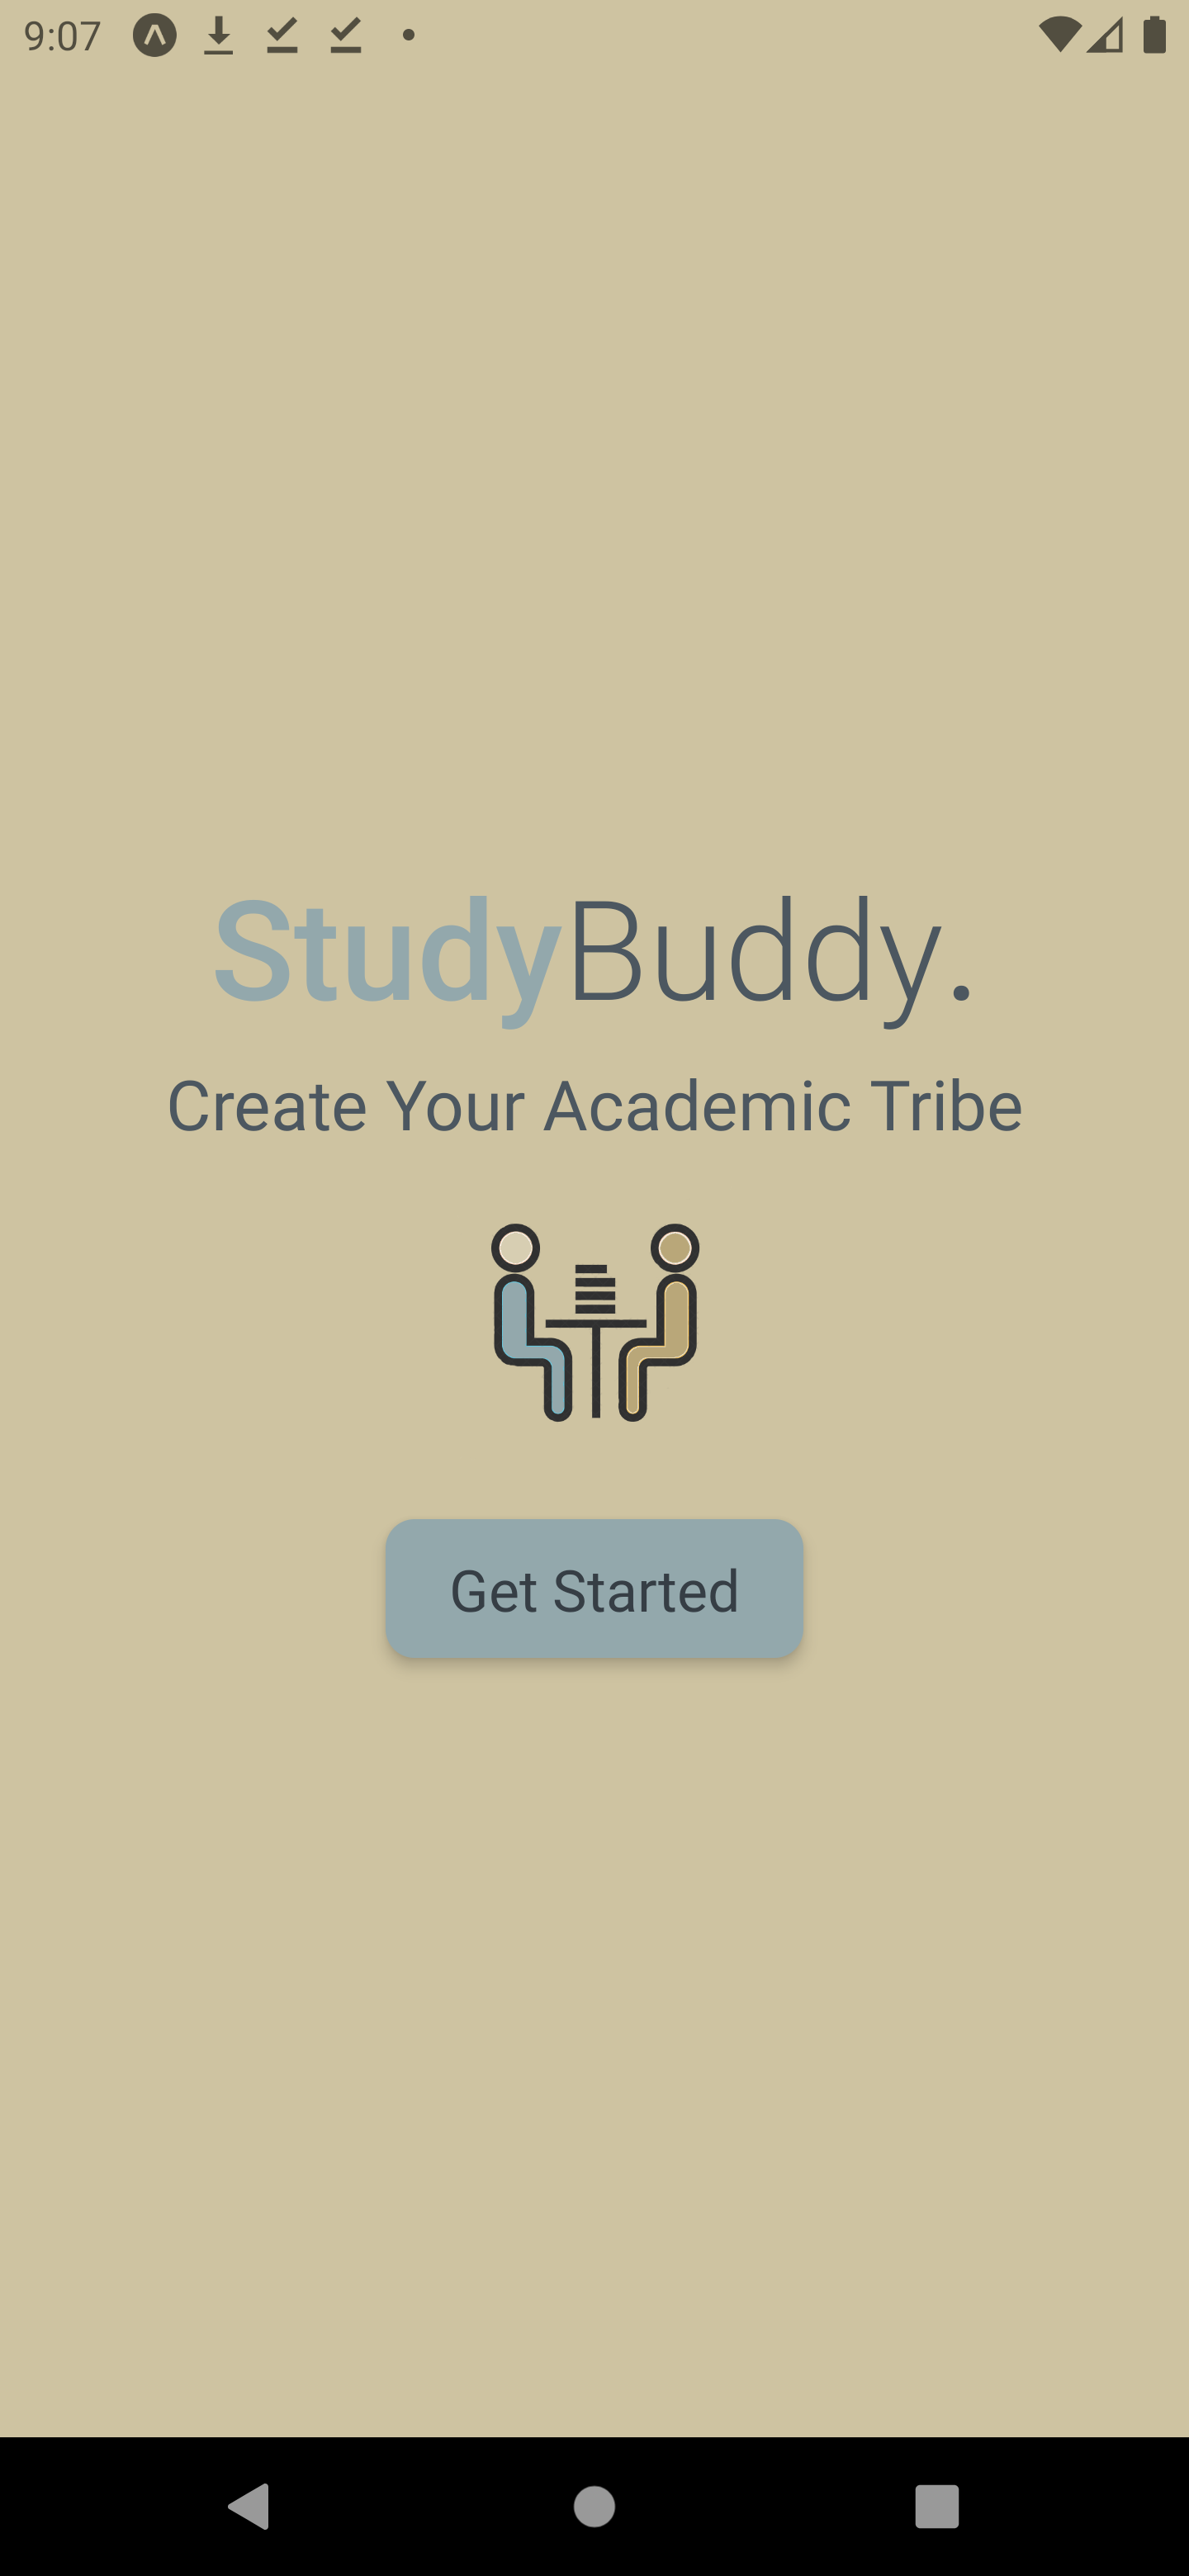
\includegraphics[width=0.45\linewidth, width=5cm, height=10cm]{images/snapshots/01.png}}
	\hspace{5pt}
	\subcaptionbox{Onboarding Slider-1}{
		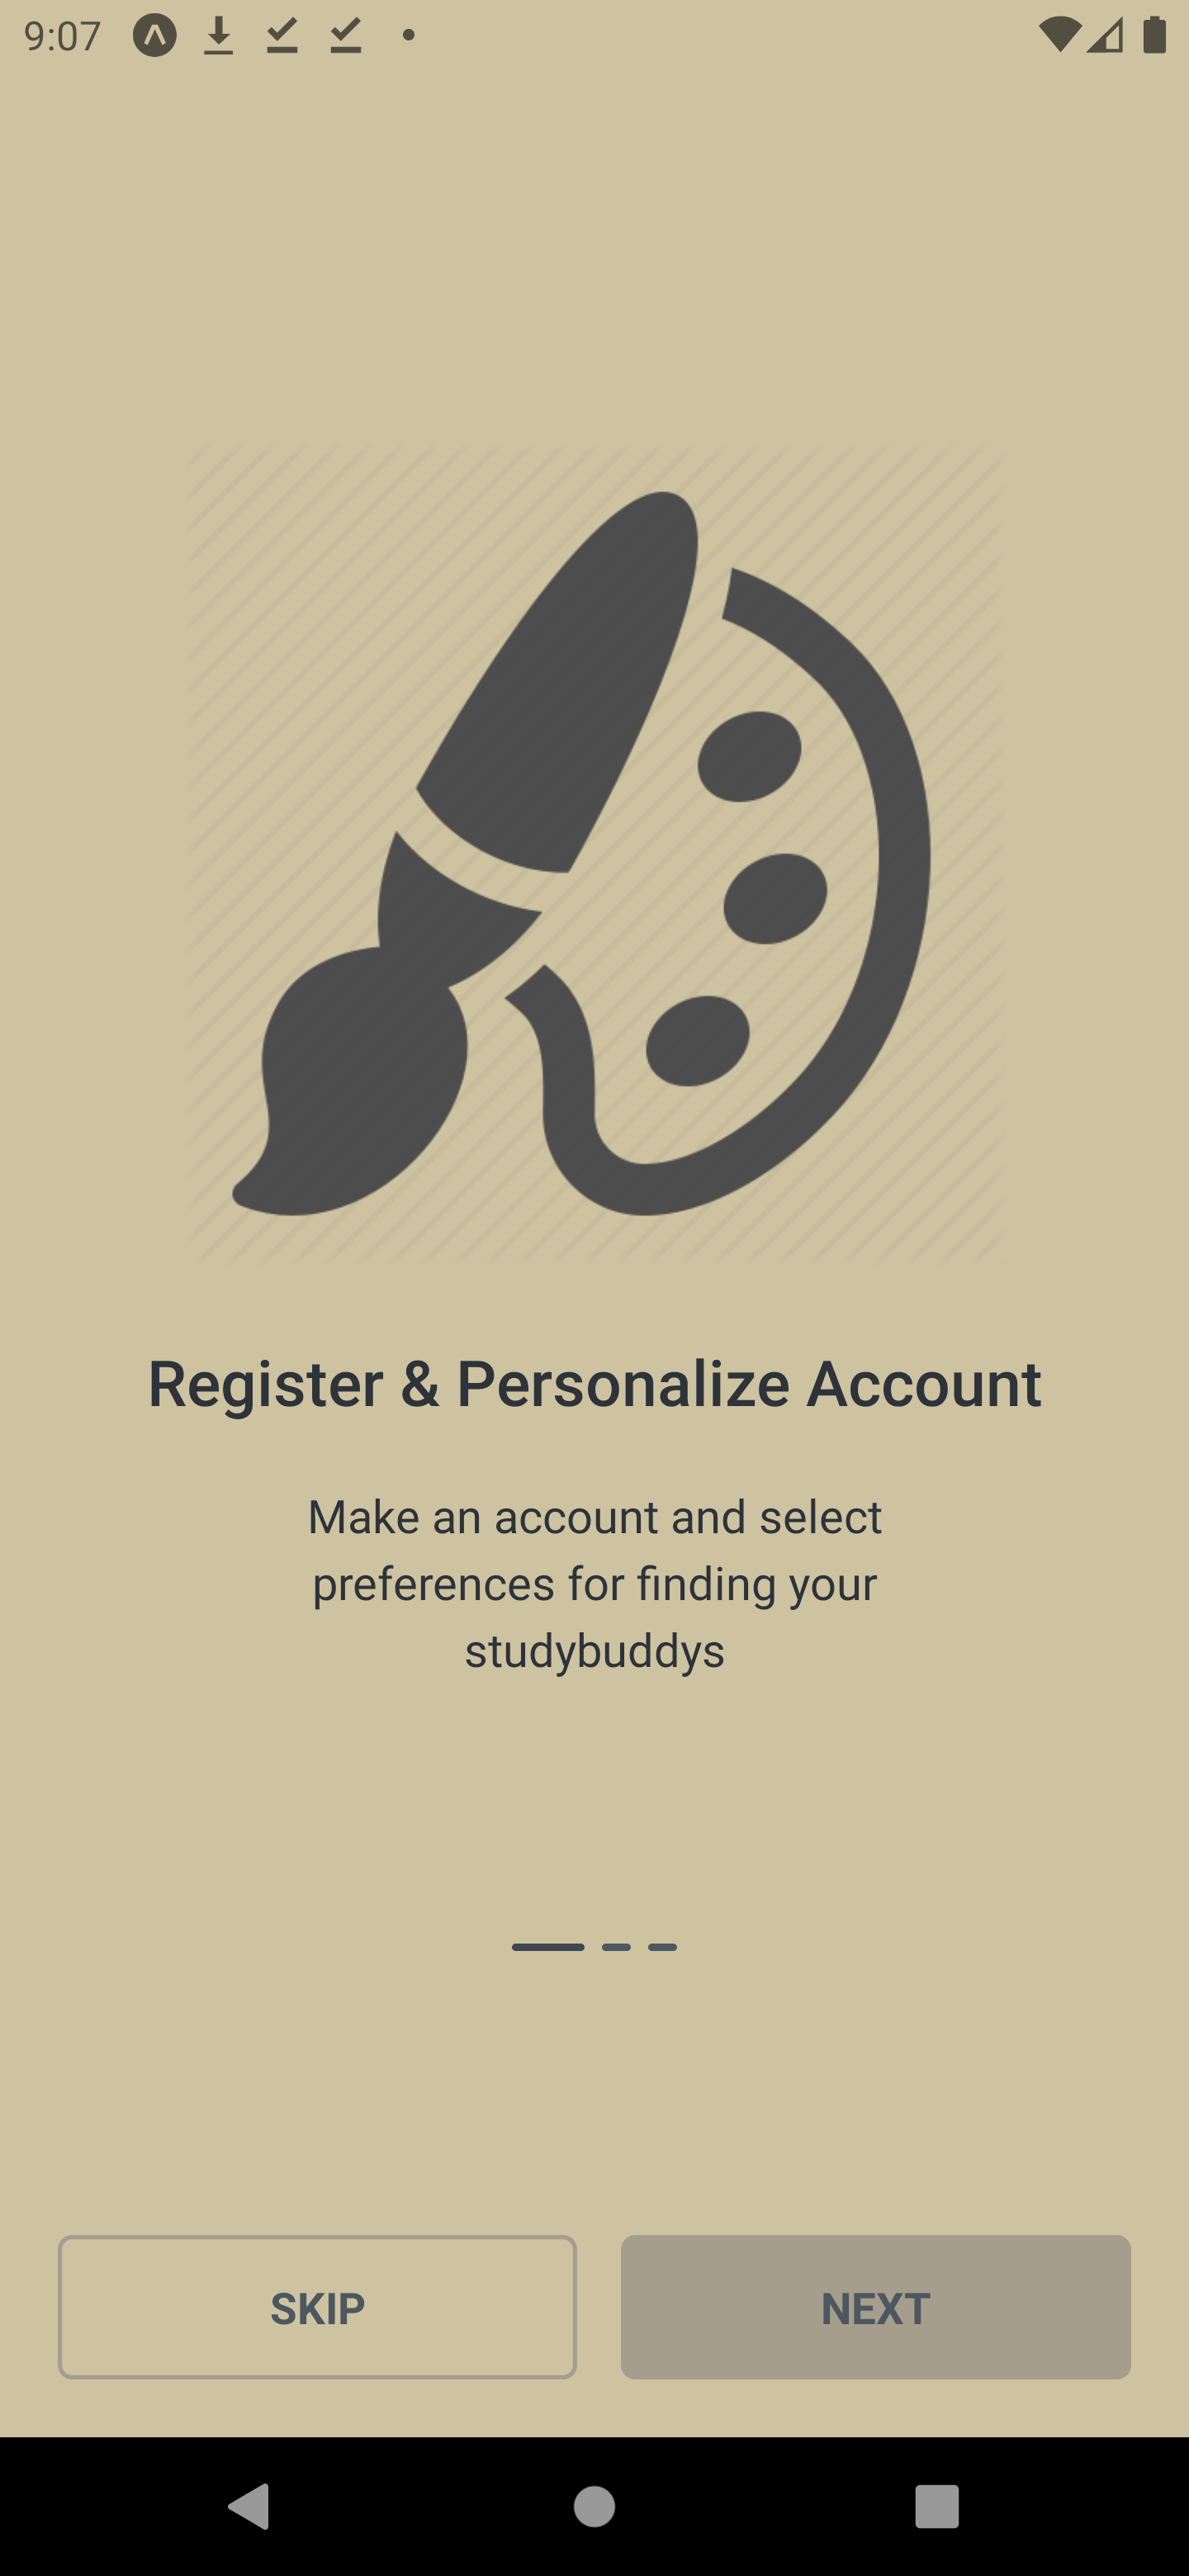
\includegraphics[width=0.45\linewidth, width=5cm, height=10cm]{images/snapshots/02.png}}
        \hspace{5pt}
	\subcaptionbox{Onboarding Slider-2}{
		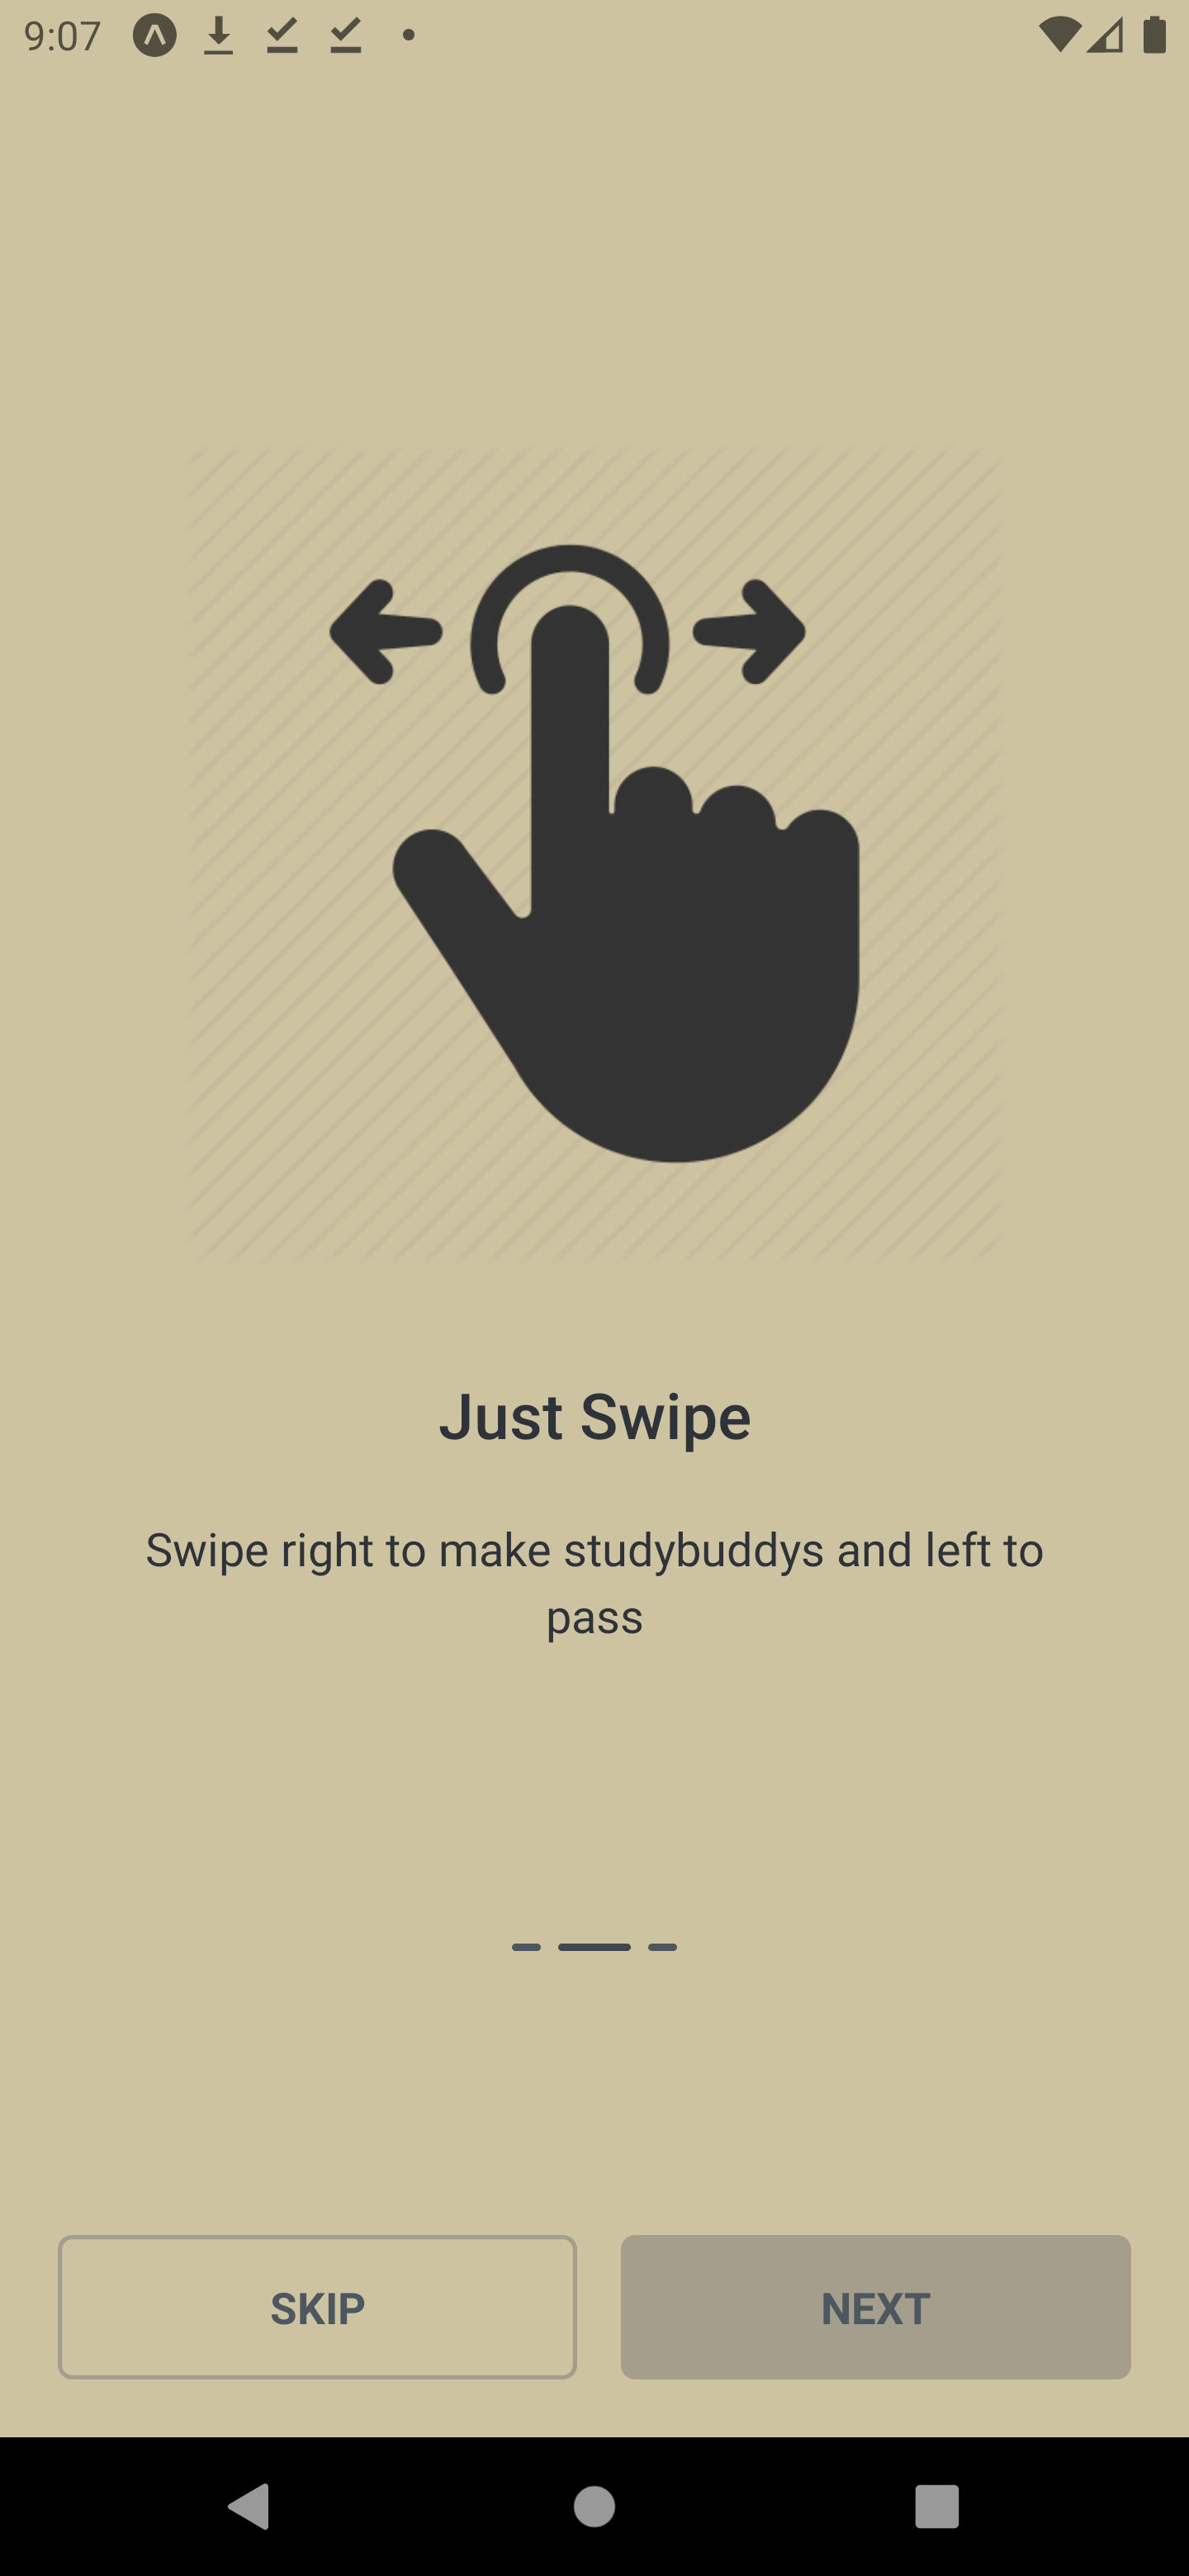
\includegraphics[width=0.45\linewidth, width=5cm, height=10cm]{images/snapshots/03.png}}
        \hspace{5pt}
	\subcaptionbox{Onboarding Slider-3}{
		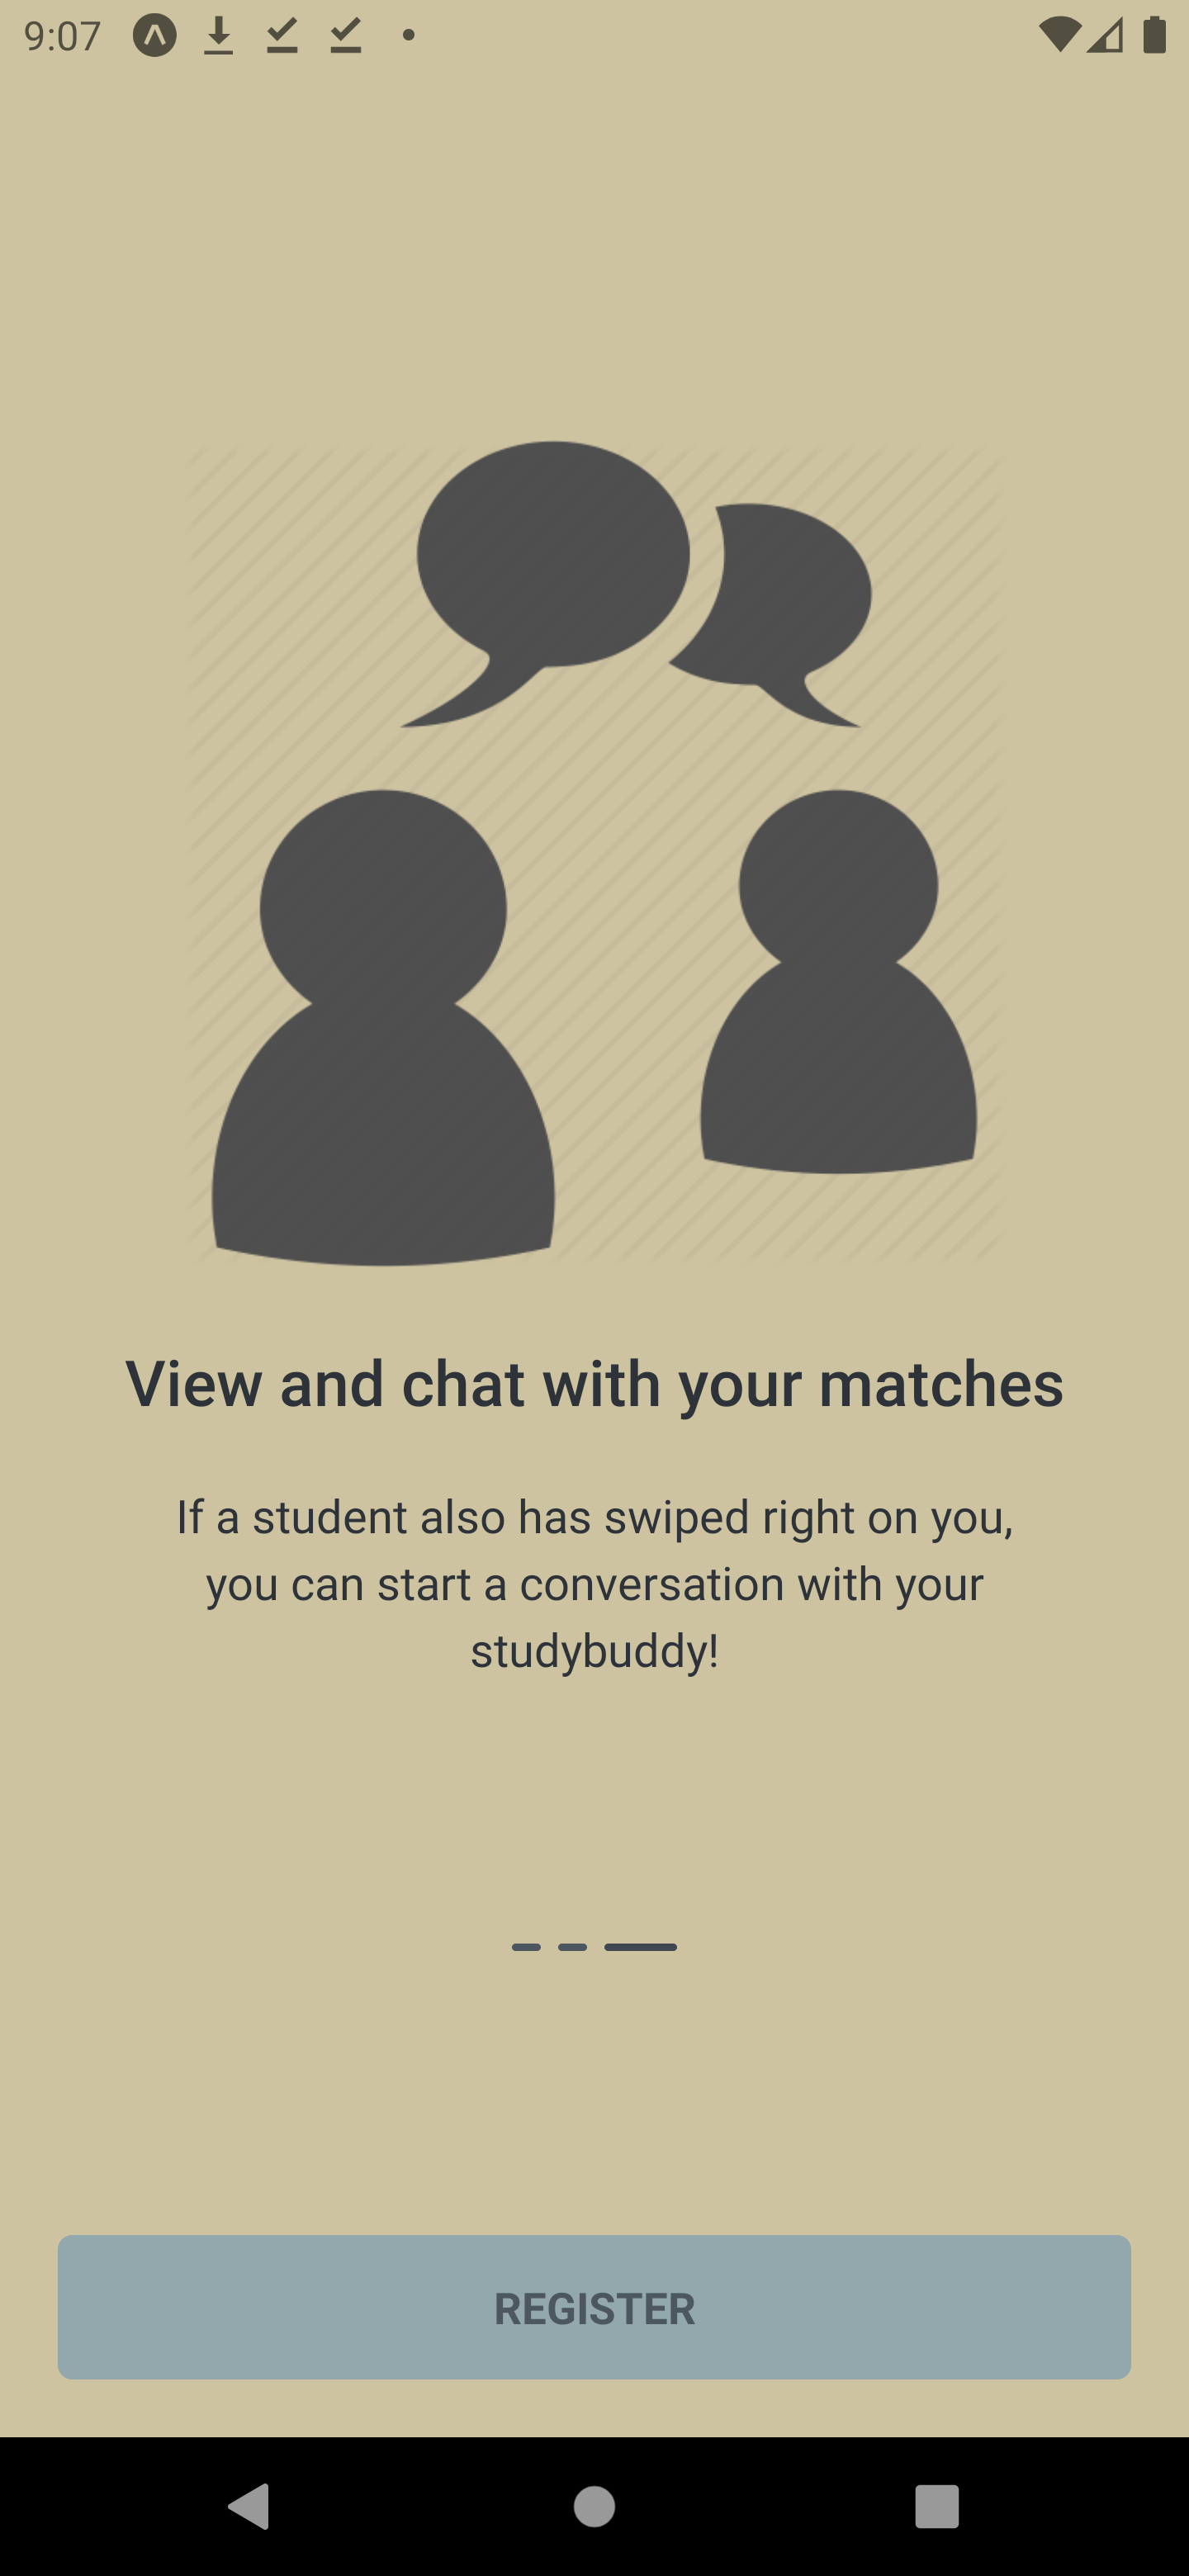
\includegraphics[width=0.45\linewidth, width=5cm, height=10cm]{images/snapshots/04.png}}
	\caption{Getting Started}
	\label{fig:get-started}
\end{figure}
\subsection{Registration and Login}
Towards the end of the Onboarding slider, users find a register button, which takes them to the registration screen. As shown in Figure~\ref{fig:authentication-screen}, if users are already registered, they can navigate to the login page. New users are required to provide a valid email, password, and full name to complete the registration process. After registration, they can log into the app. At the registration page, users can also view terms and conditions which are mentioned in detail in section~\ref{sec:tnc}.
  \begin{figure}[H]
	\centering
	\subcaptionbox{Registration Screen}{
		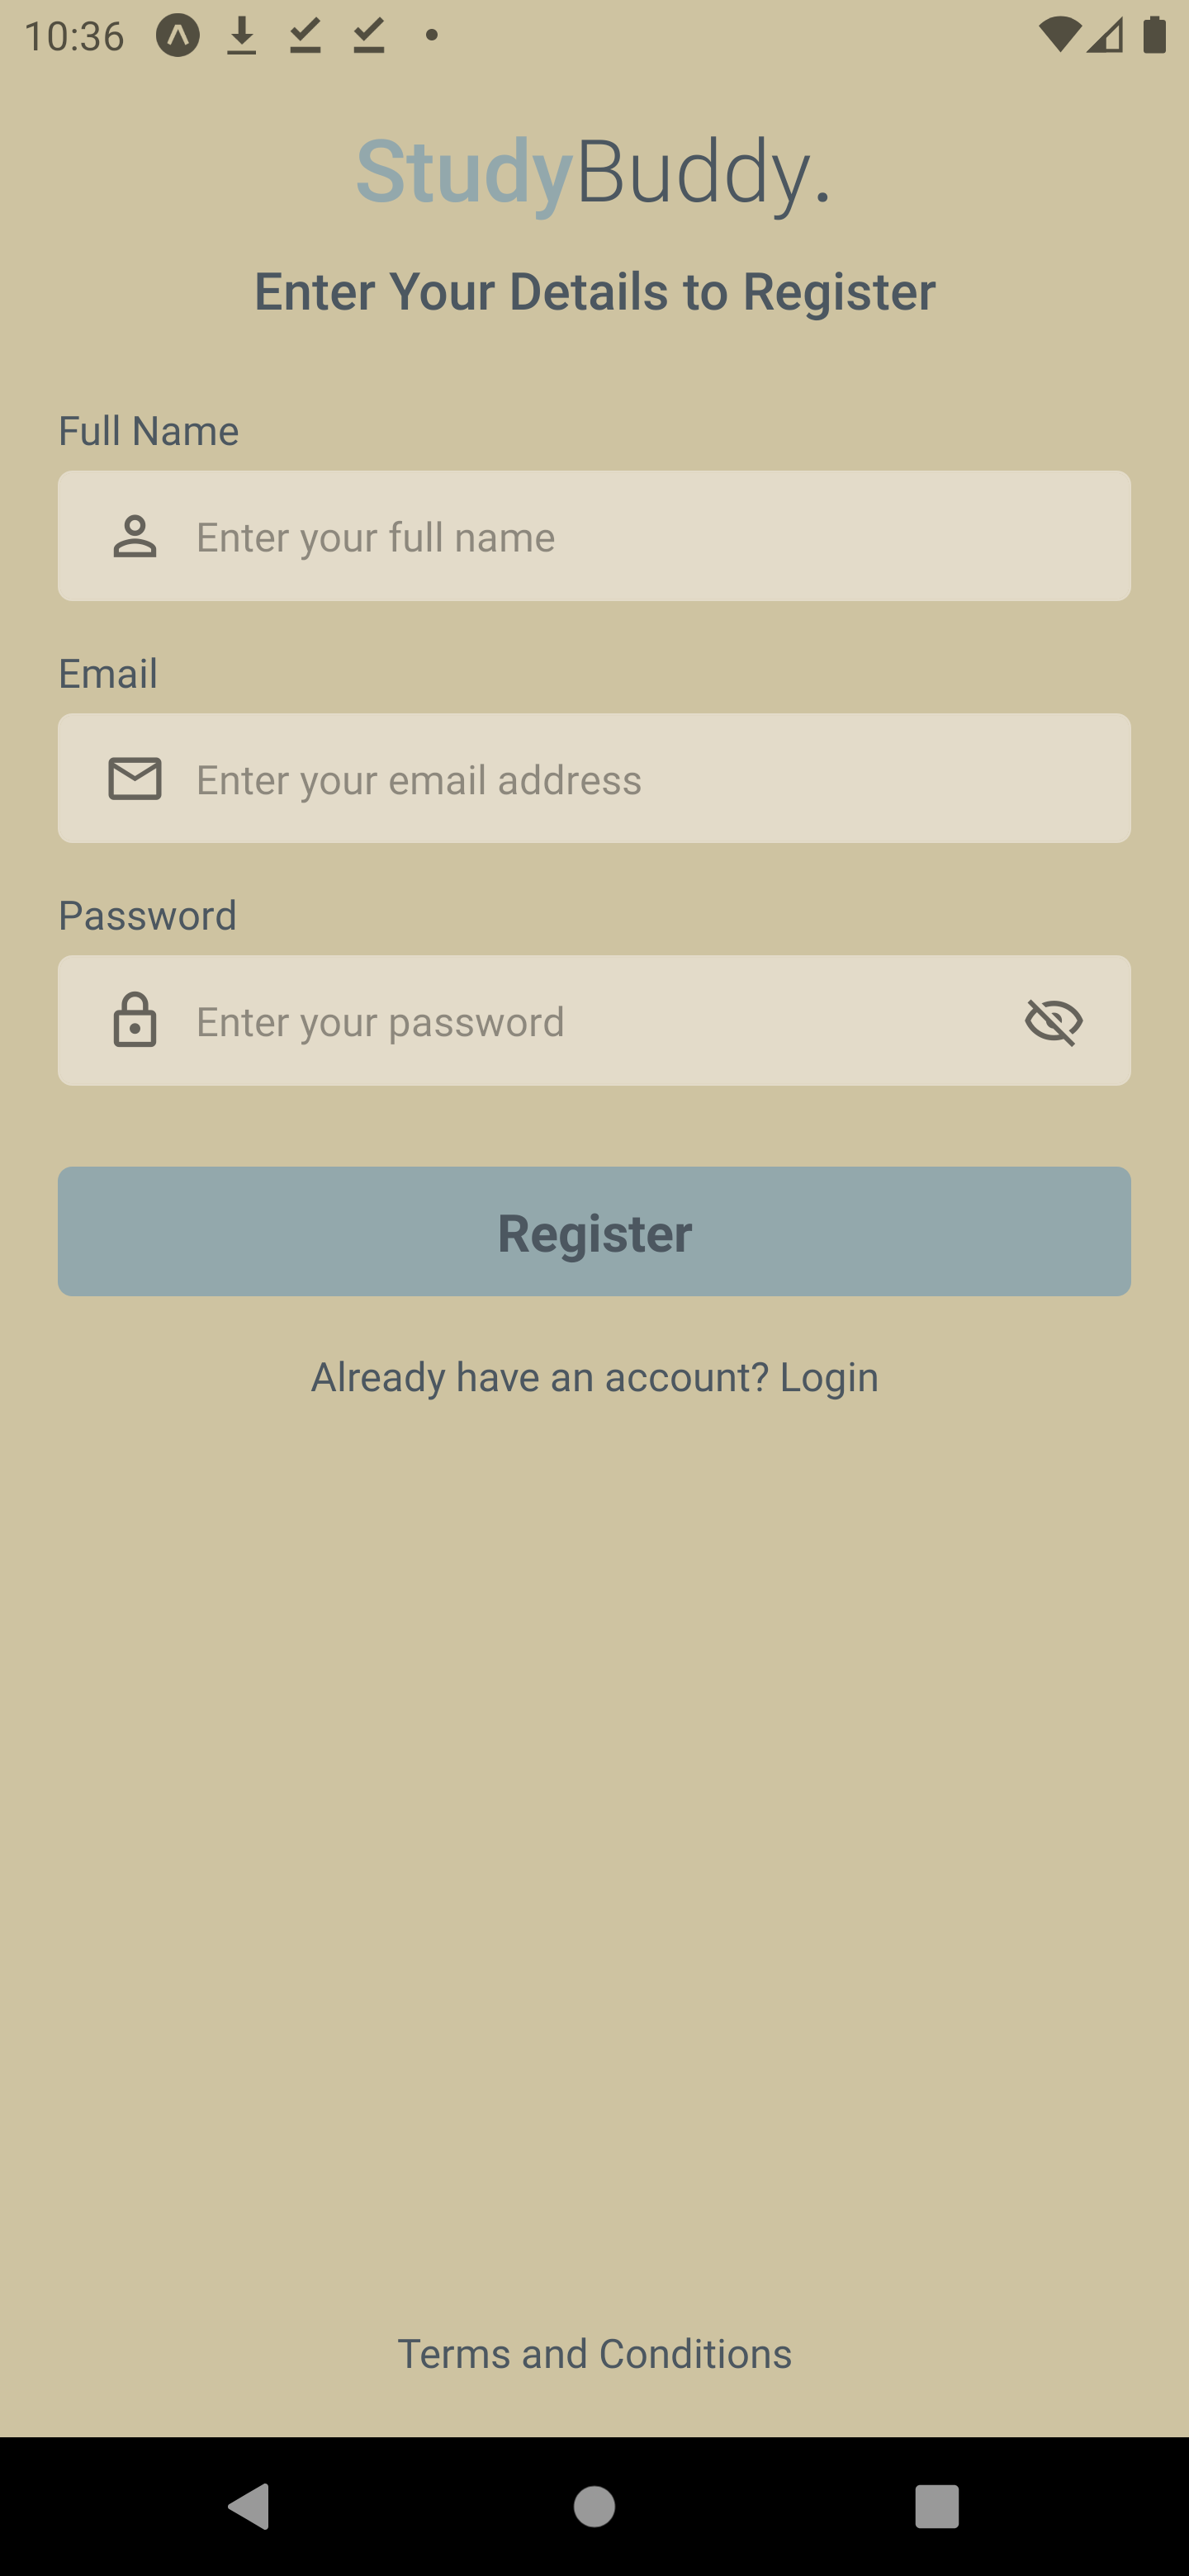
\includegraphics[width=0.45\linewidth, width=5cm, height=10cm]{images/snapshots/register.png}}
	\hspace{5pt}
	\subcaptionbox{Login Screen}{
		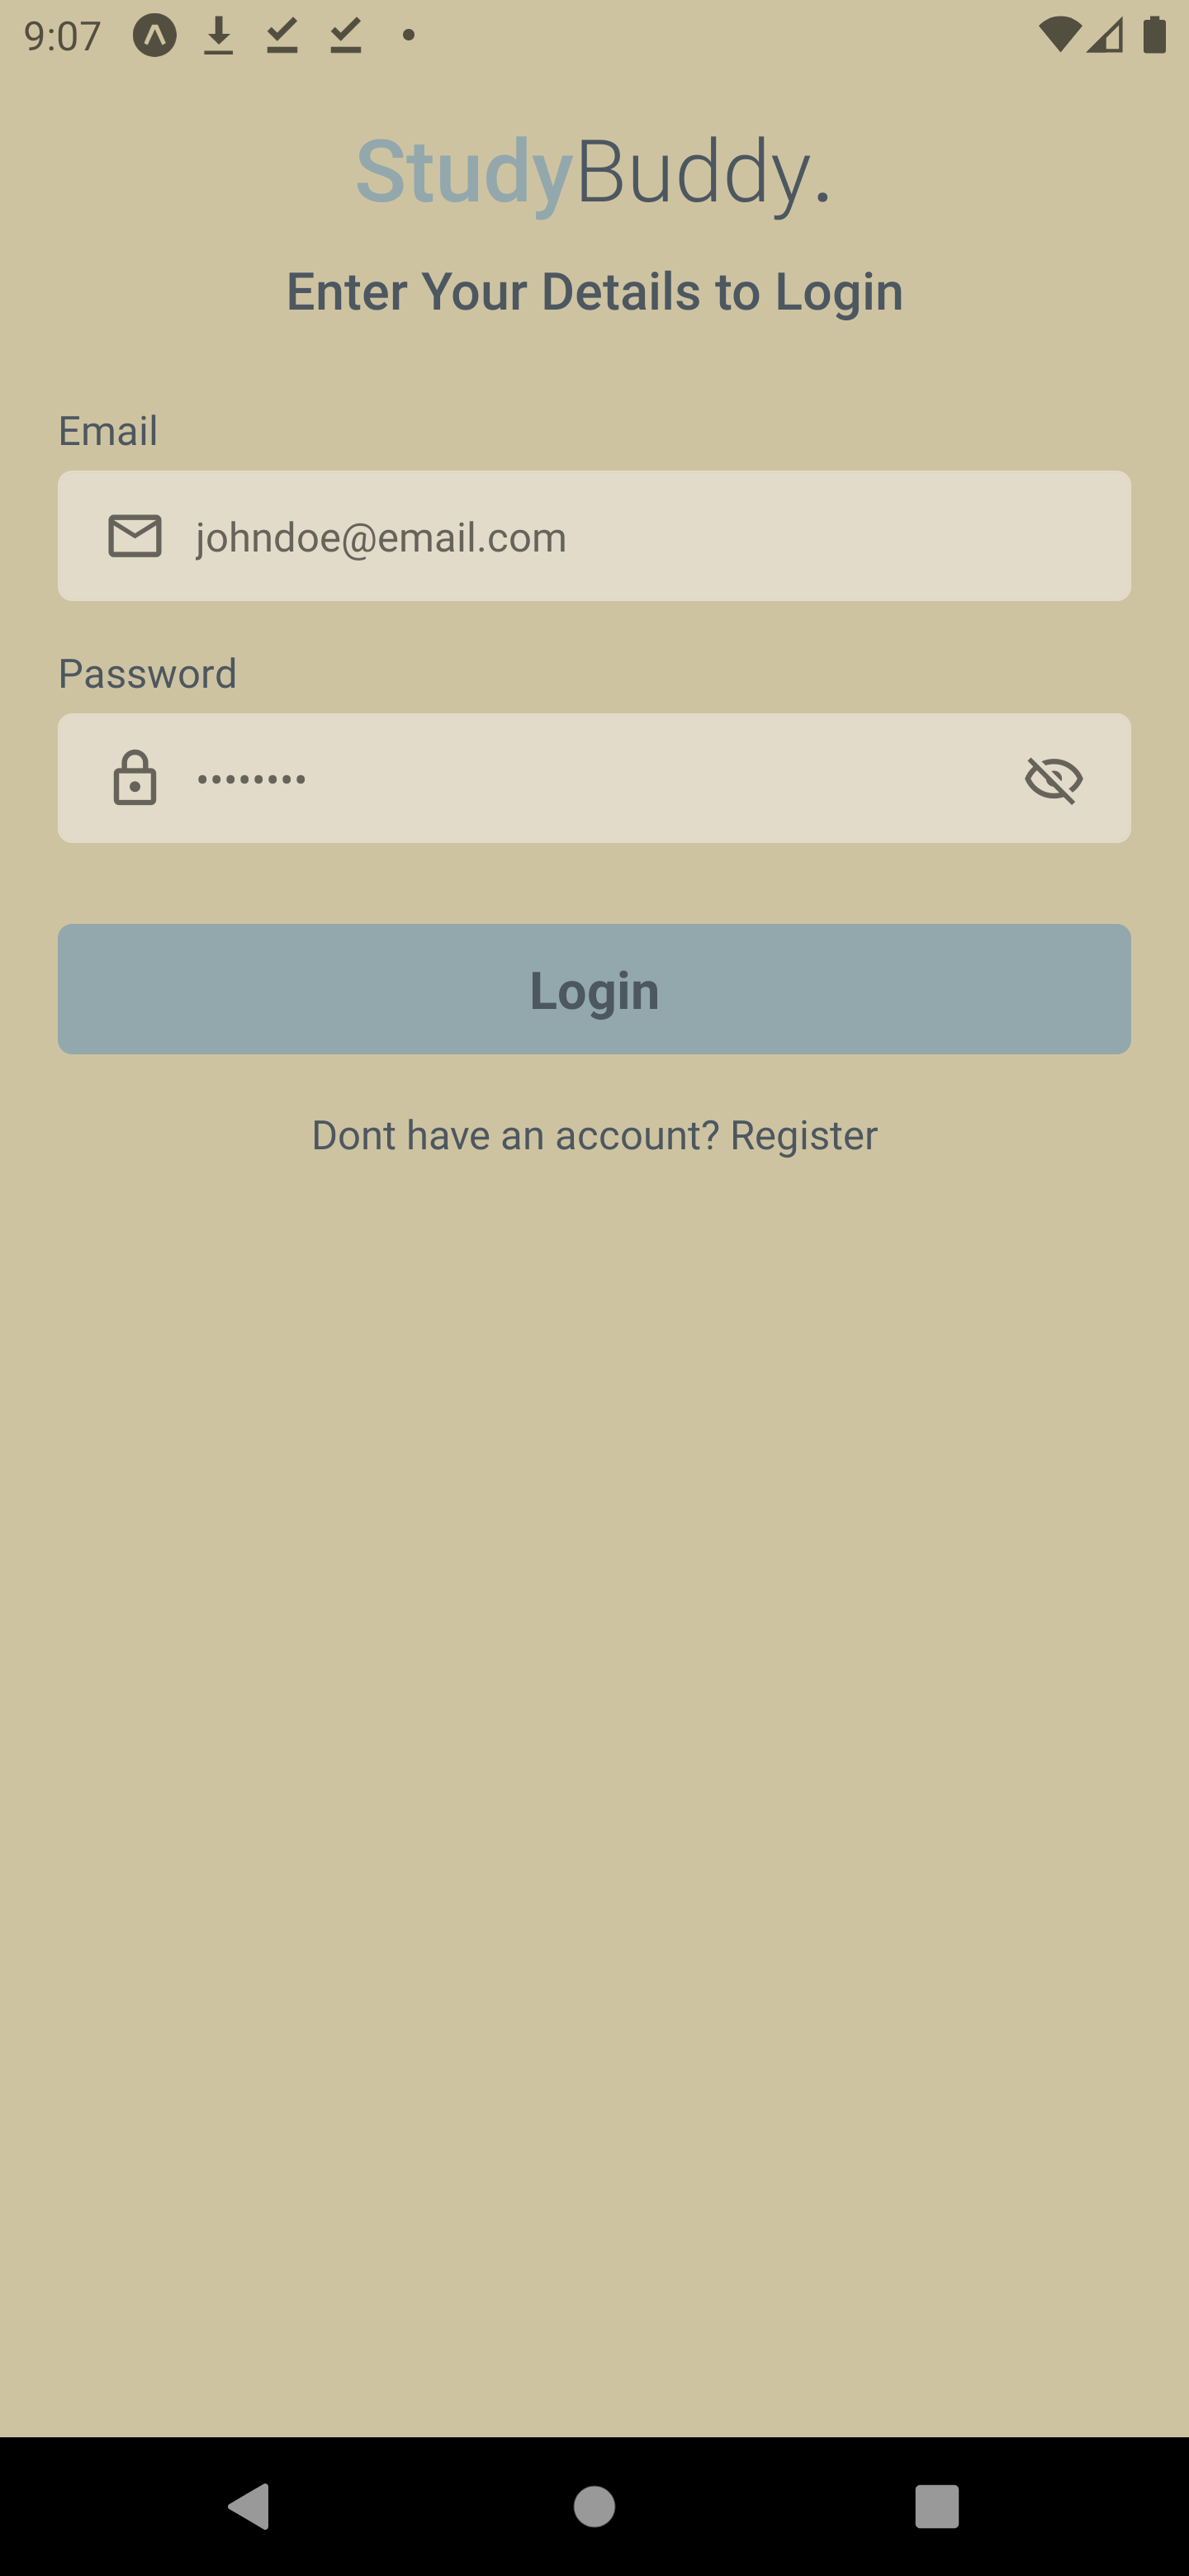
\includegraphics[width=0.45\linewidth, width=5cm, height=10cm]{images/snapshots/06.png}}
	\caption{Authentication}
	\label{fig:authentication-screen}
\end{figure}
\subsection{Complete Profile}
After login, users are directed to the complete profile section. They need to provide specific information, such as selecting up to four languages and courses, their university, major and city. These selections are mandatory for moving forward and are mentioned with asterisk as shown in Figure~\ref{fig:complete-profile-screen}. Upon submission, users are navigated to the home screen.
   \begin{figure}[H]
	\centering
	\subcaptionbox{Edit Profile}{
		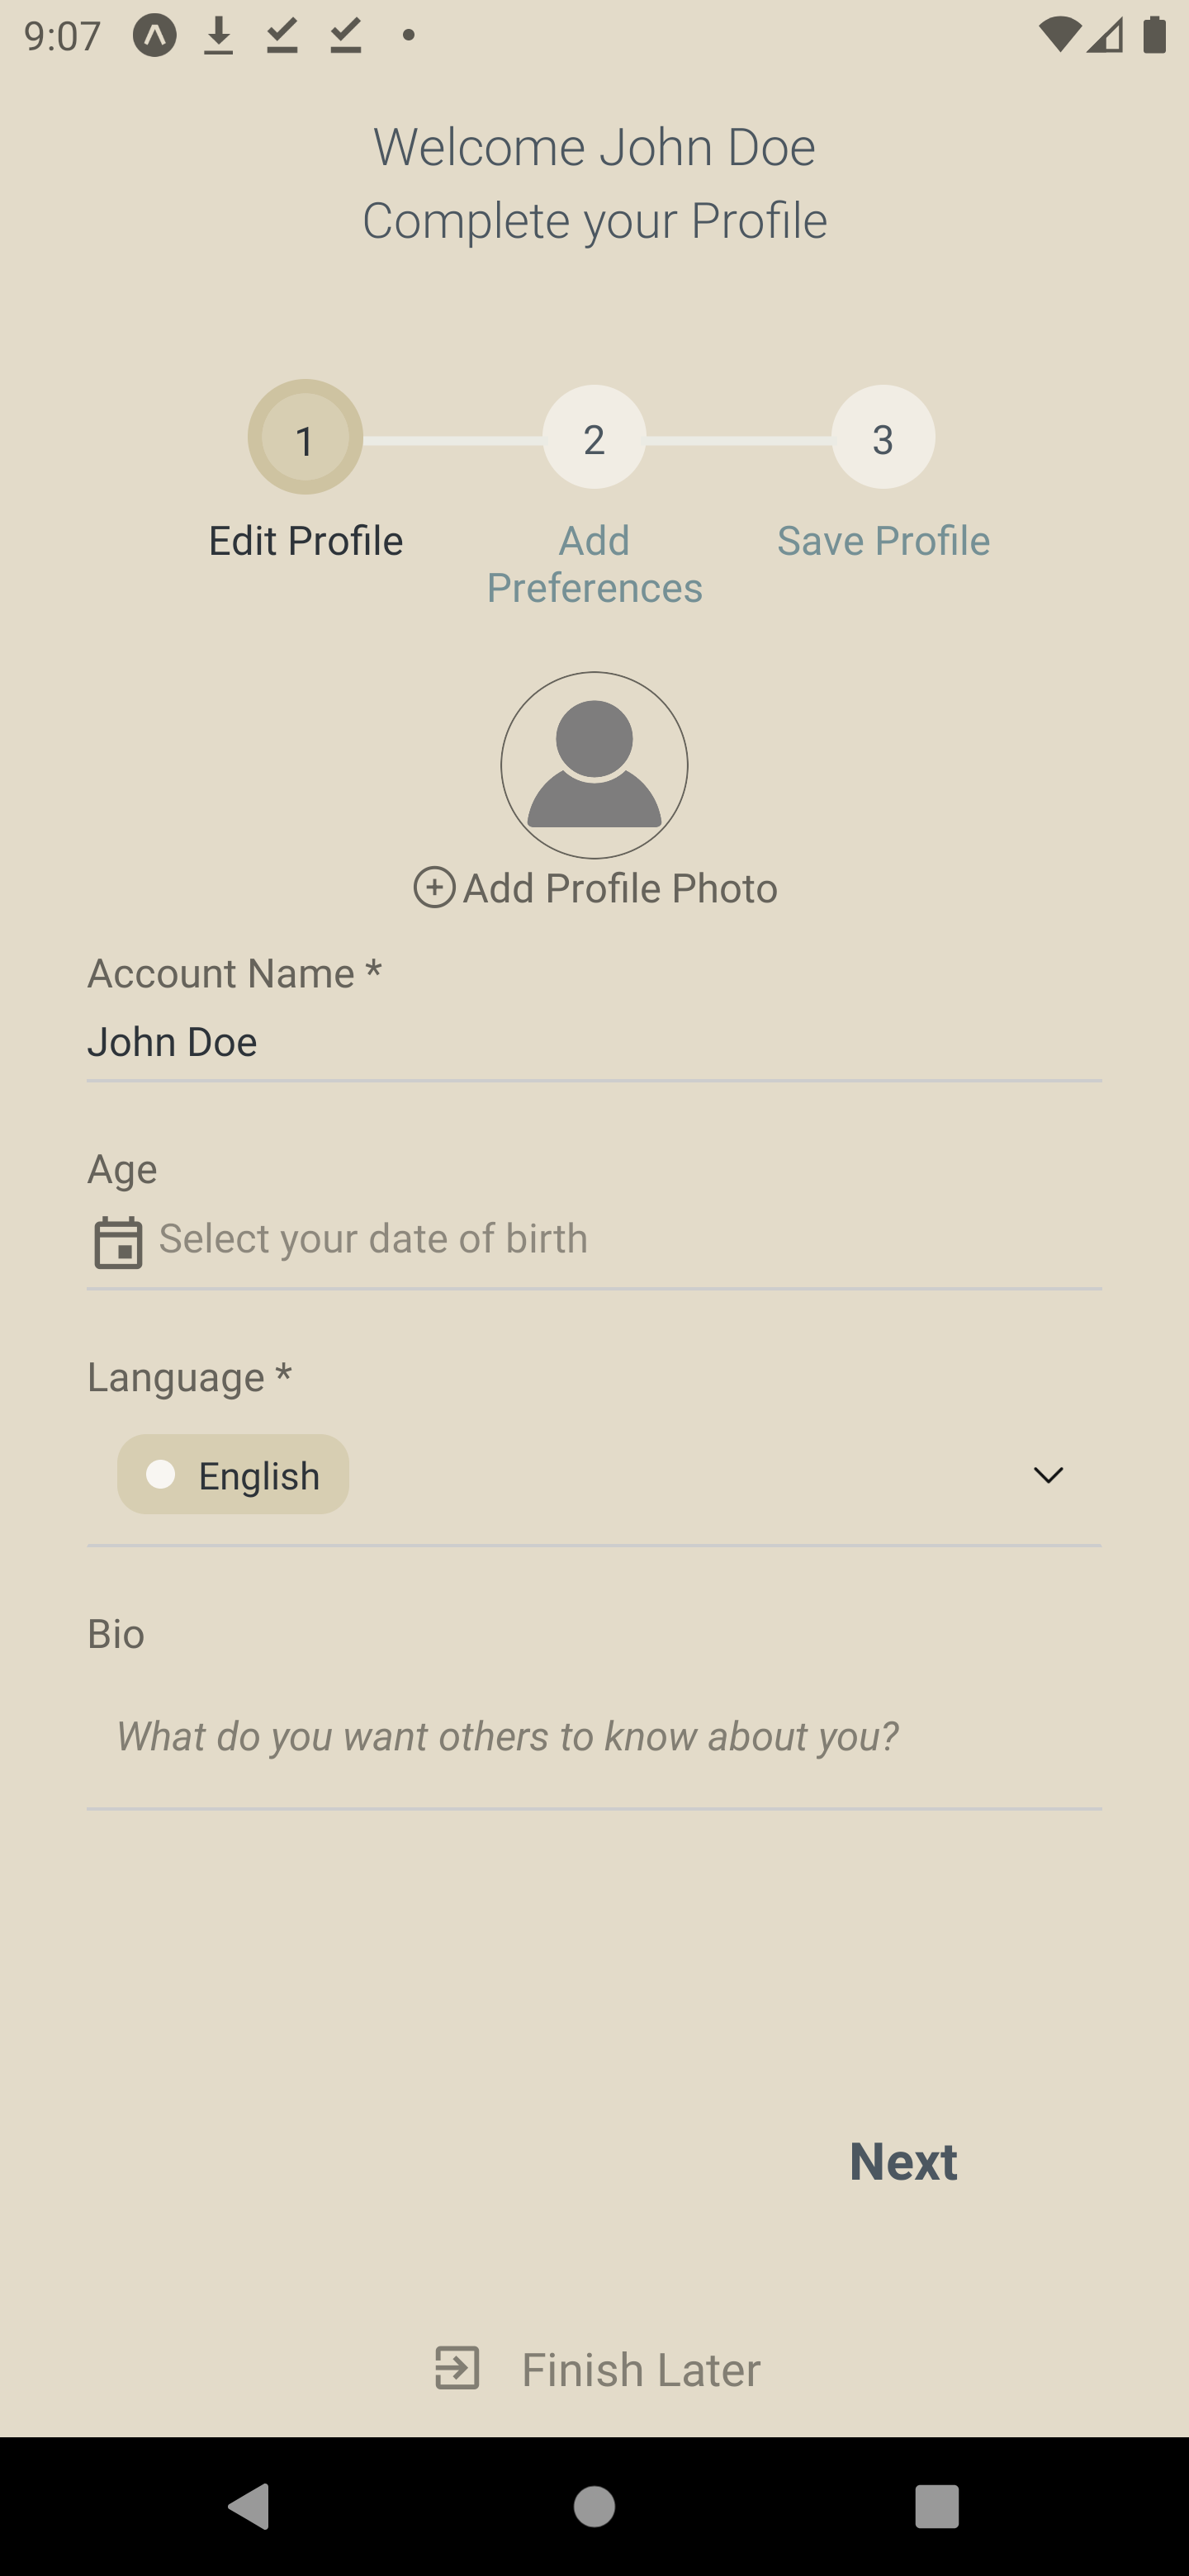
\includegraphics[width=0.45\linewidth, width=5cm, height=10cm]{images/snapshots/07.png}}
	\hspace{5pt}
	\subcaptionbox{Add Preferences}{
		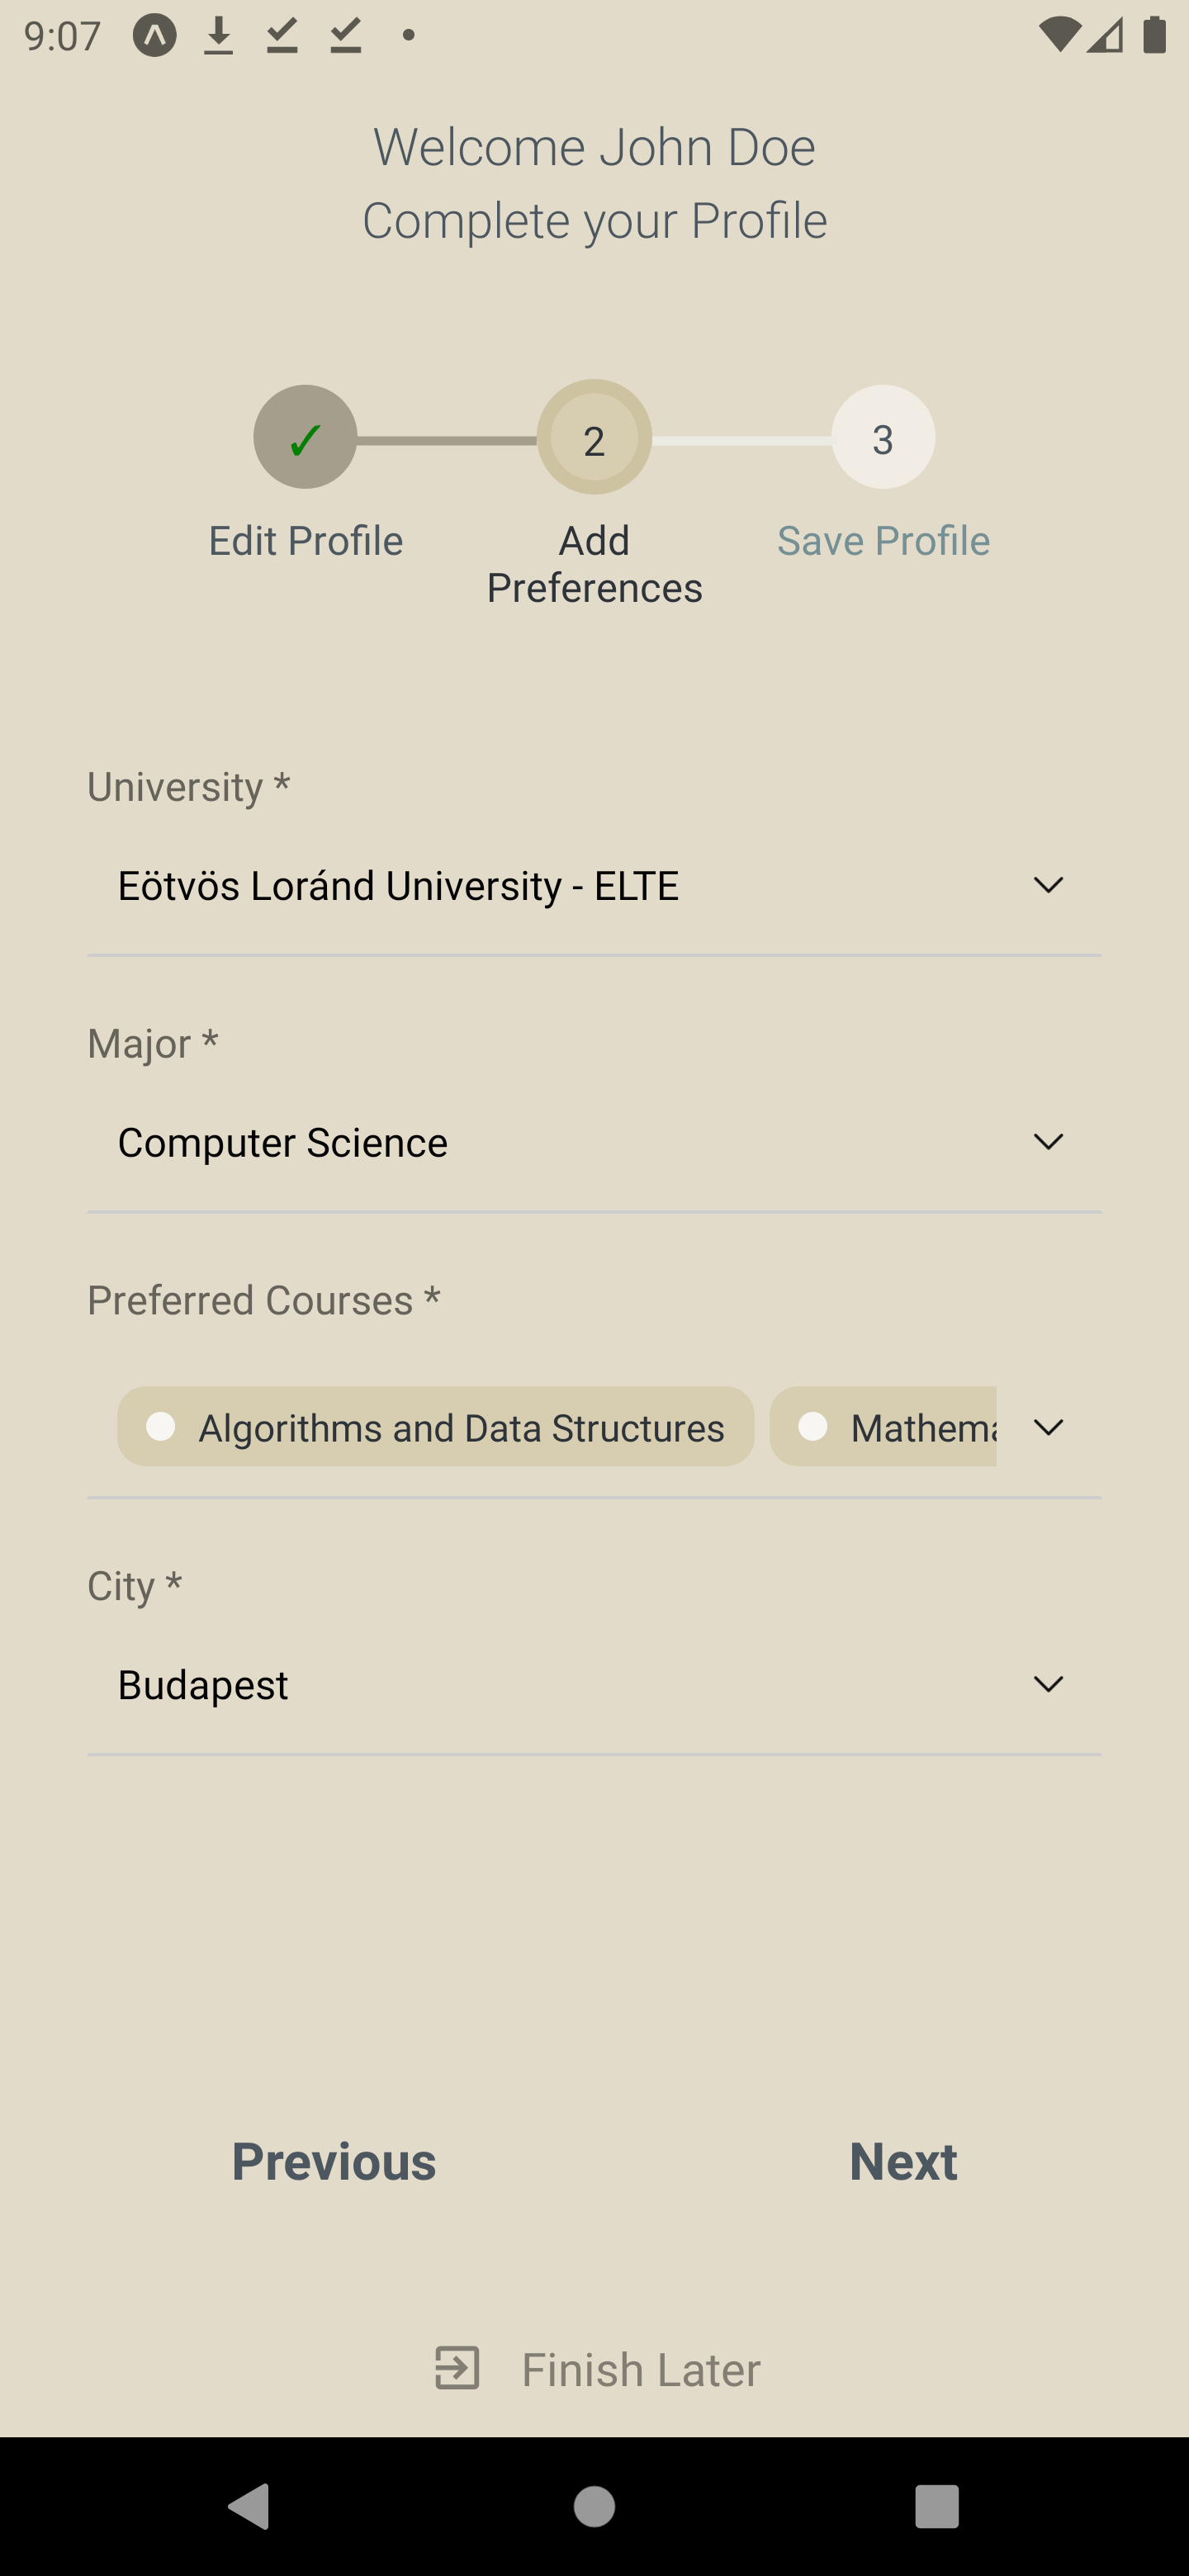
\includegraphics[width=0.45\linewidth, width=5cm, height=10cm]{images/snapshots/08.png}}
	\hspace{5pt}
	\subcaptionbox{Submit Details}{
		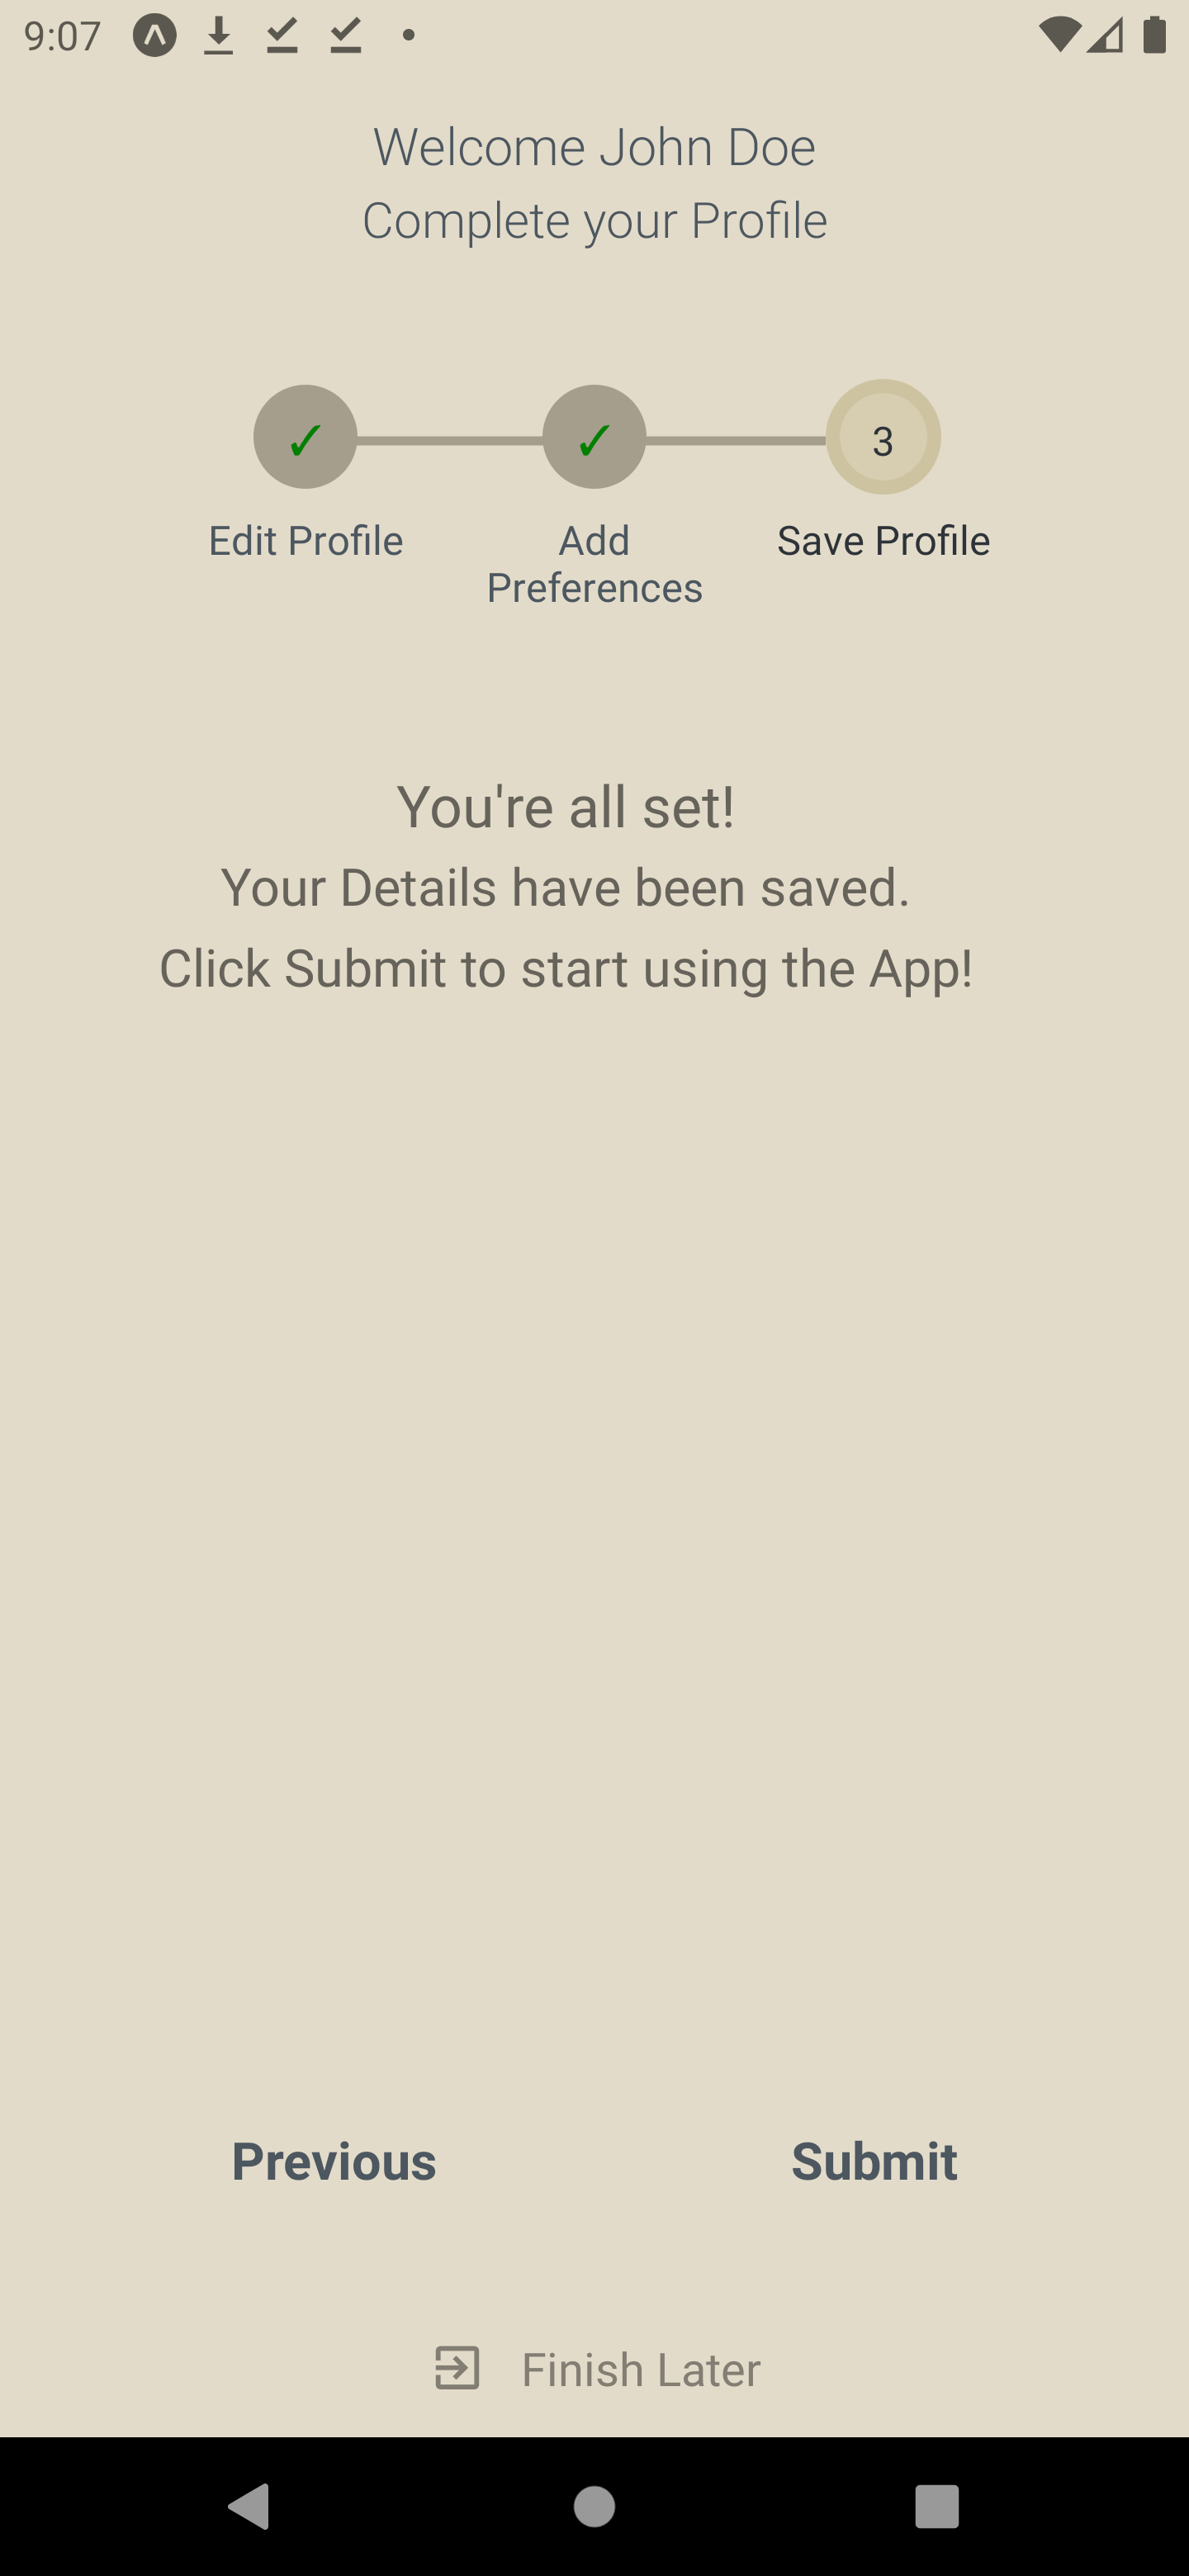
\includegraphics[width=0.45\linewidth, width=5cm, height=10cm]{images/snapshots/09.png}}
	\caption{Complete Profile Screen}
	\label{fig:complete-profile-screen}
\end{figure}
\subsection{Home Screen and Swipe Functionality}
The home screen is the central hub of the app. Users can view other app users as cards that can be swiped left or right. Each card is accompanied by a user info modal at the bottom, displaying additional information for each user as shown in Figure~\ref{fig:home-screen}. Users can also check recommendation scores for each other that is implemented by OpenAI API (see section~\ref{subsec:recommendations}). Users can swipe left or right (see figure~\ref{fig:swiping}) on the cards or tap the like/dislike buttons represented by thumbs up or thumbs down icons. Once all users have been swiped, the buttons are disabled, and no more cards are shown. 
 \begin{figure}[H]
	\centering
	\subcaptionbox{Home Screen}{
		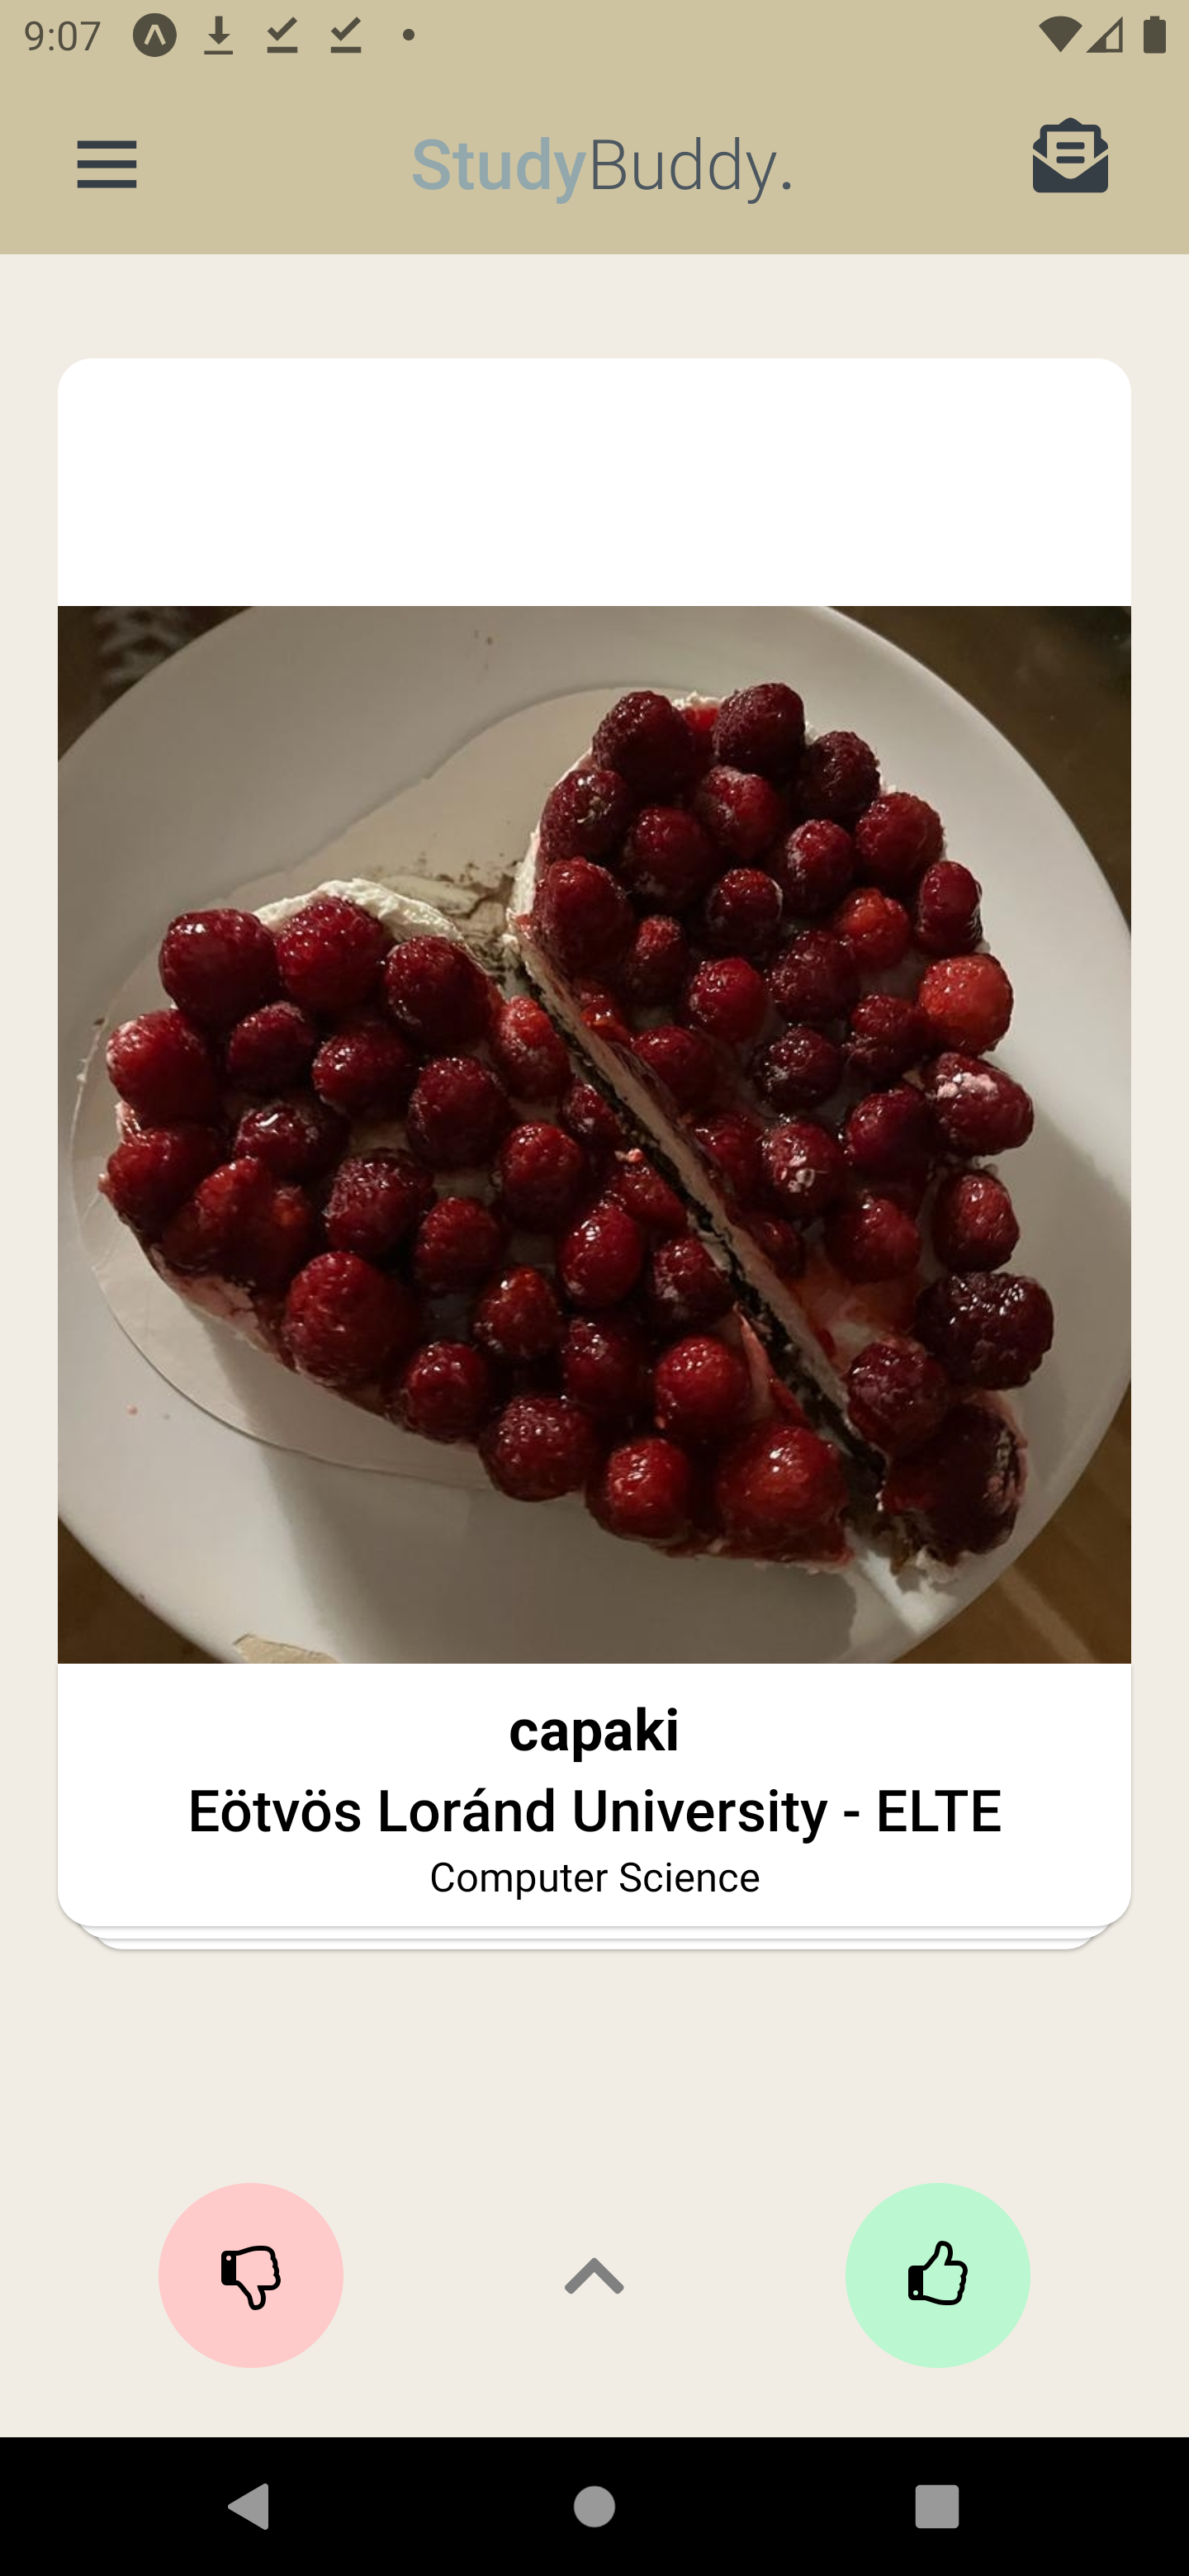
\includegraphics[width=0.45\linewidth, width=5cm, height=10cm]{images/snapshots/10.png}}
	\hspace{5pt}
	\subcaptionbox{User Info Modal}{
		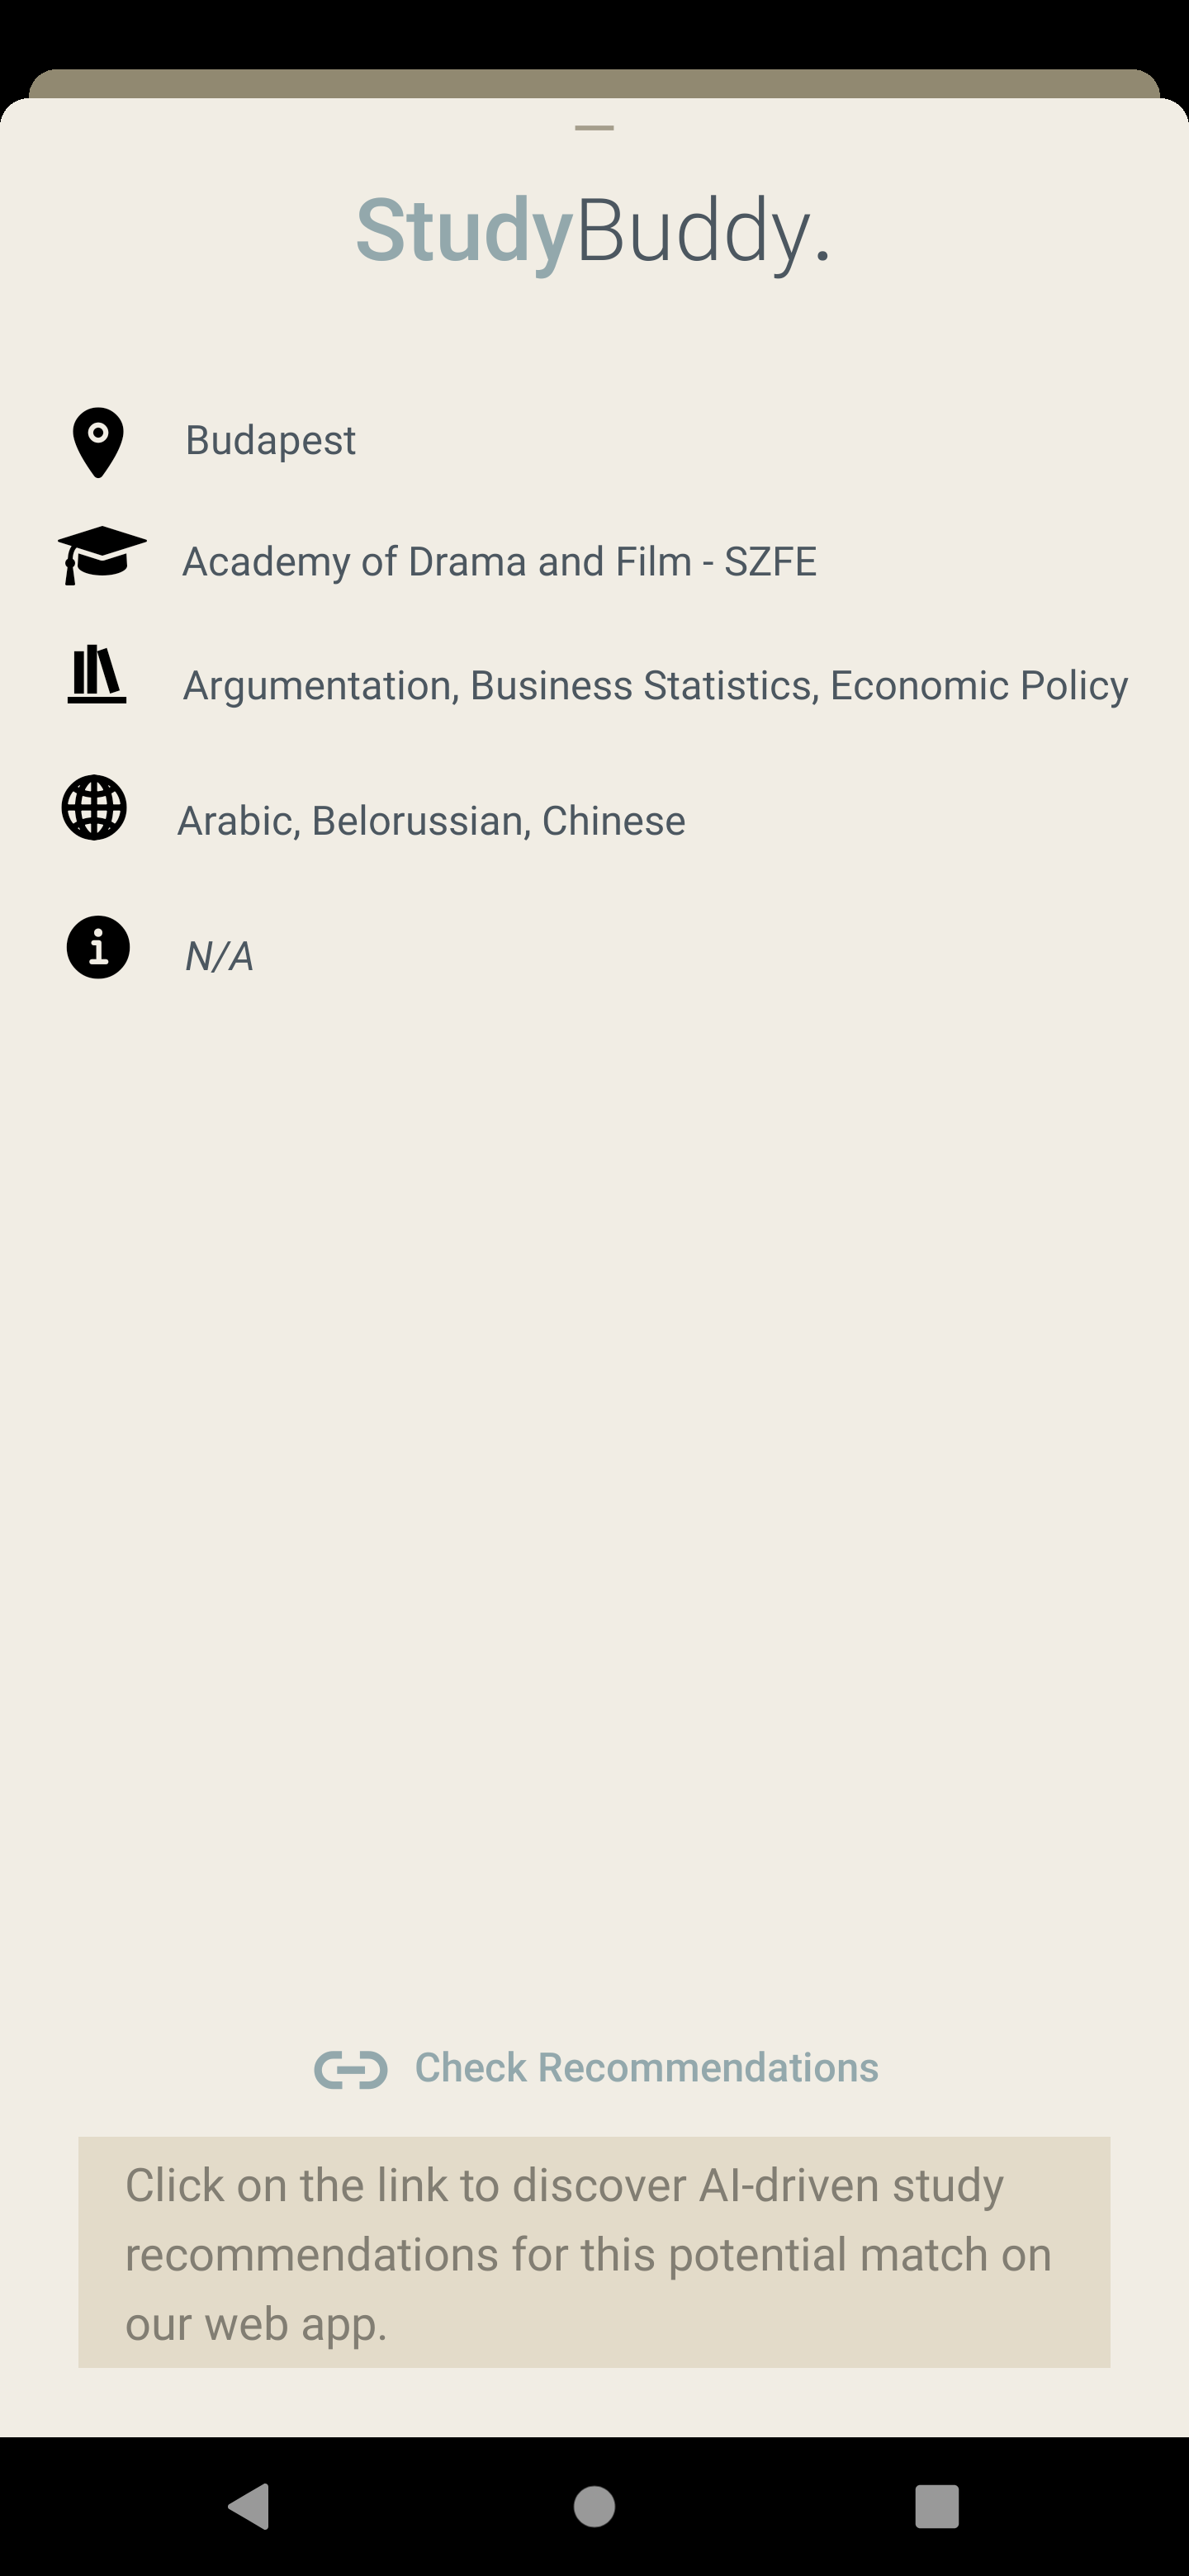
\includegraphics[width=0.45\linewidth, width=5cm, height=10cm]{images/snapshots/userinfomodal.png}}
	\caption{Home Screen}
	\label{fig:home-screen}
\end{figure}
\begin{figure}[H]
	\centering
  \subcaptionbox{Swiping}{
		
\includegraphics[width=0.45\linewidth, width=5cm, height=7cm]{images/snapshots/11.png}}
	\caption{Home Screen}
	\label{fig:swiping}
\end{figure}
\subsection{Recommendations}\label{subsec:recommendations}
Users can conveniently check their recommendation scores by accessing the admin web app of our mobile application. The recommendation scores, provided by the OpenAI API, are displayed on a web page accessible through a unique link. The scores are given on a scale of ten, allowing users to gauge the relevance and suitability of recommendations for their specific needs.

In the event of any unforeseen slowdown or error in the OpenAI API, our web page incorporates an error handler as shown in figure~\ref{fig:recommend}. This ensures a seamless user experience by promptly addressing and communicating any temporary disruptions. We strive to minimize any impact on the accessibility and accuracy of the recommendation scores, providing users with reliable and valuable insights through our admin web app.
   \begin{figure}[H]
	\centering
	\subcaptionbox{Recommendation Score}{
		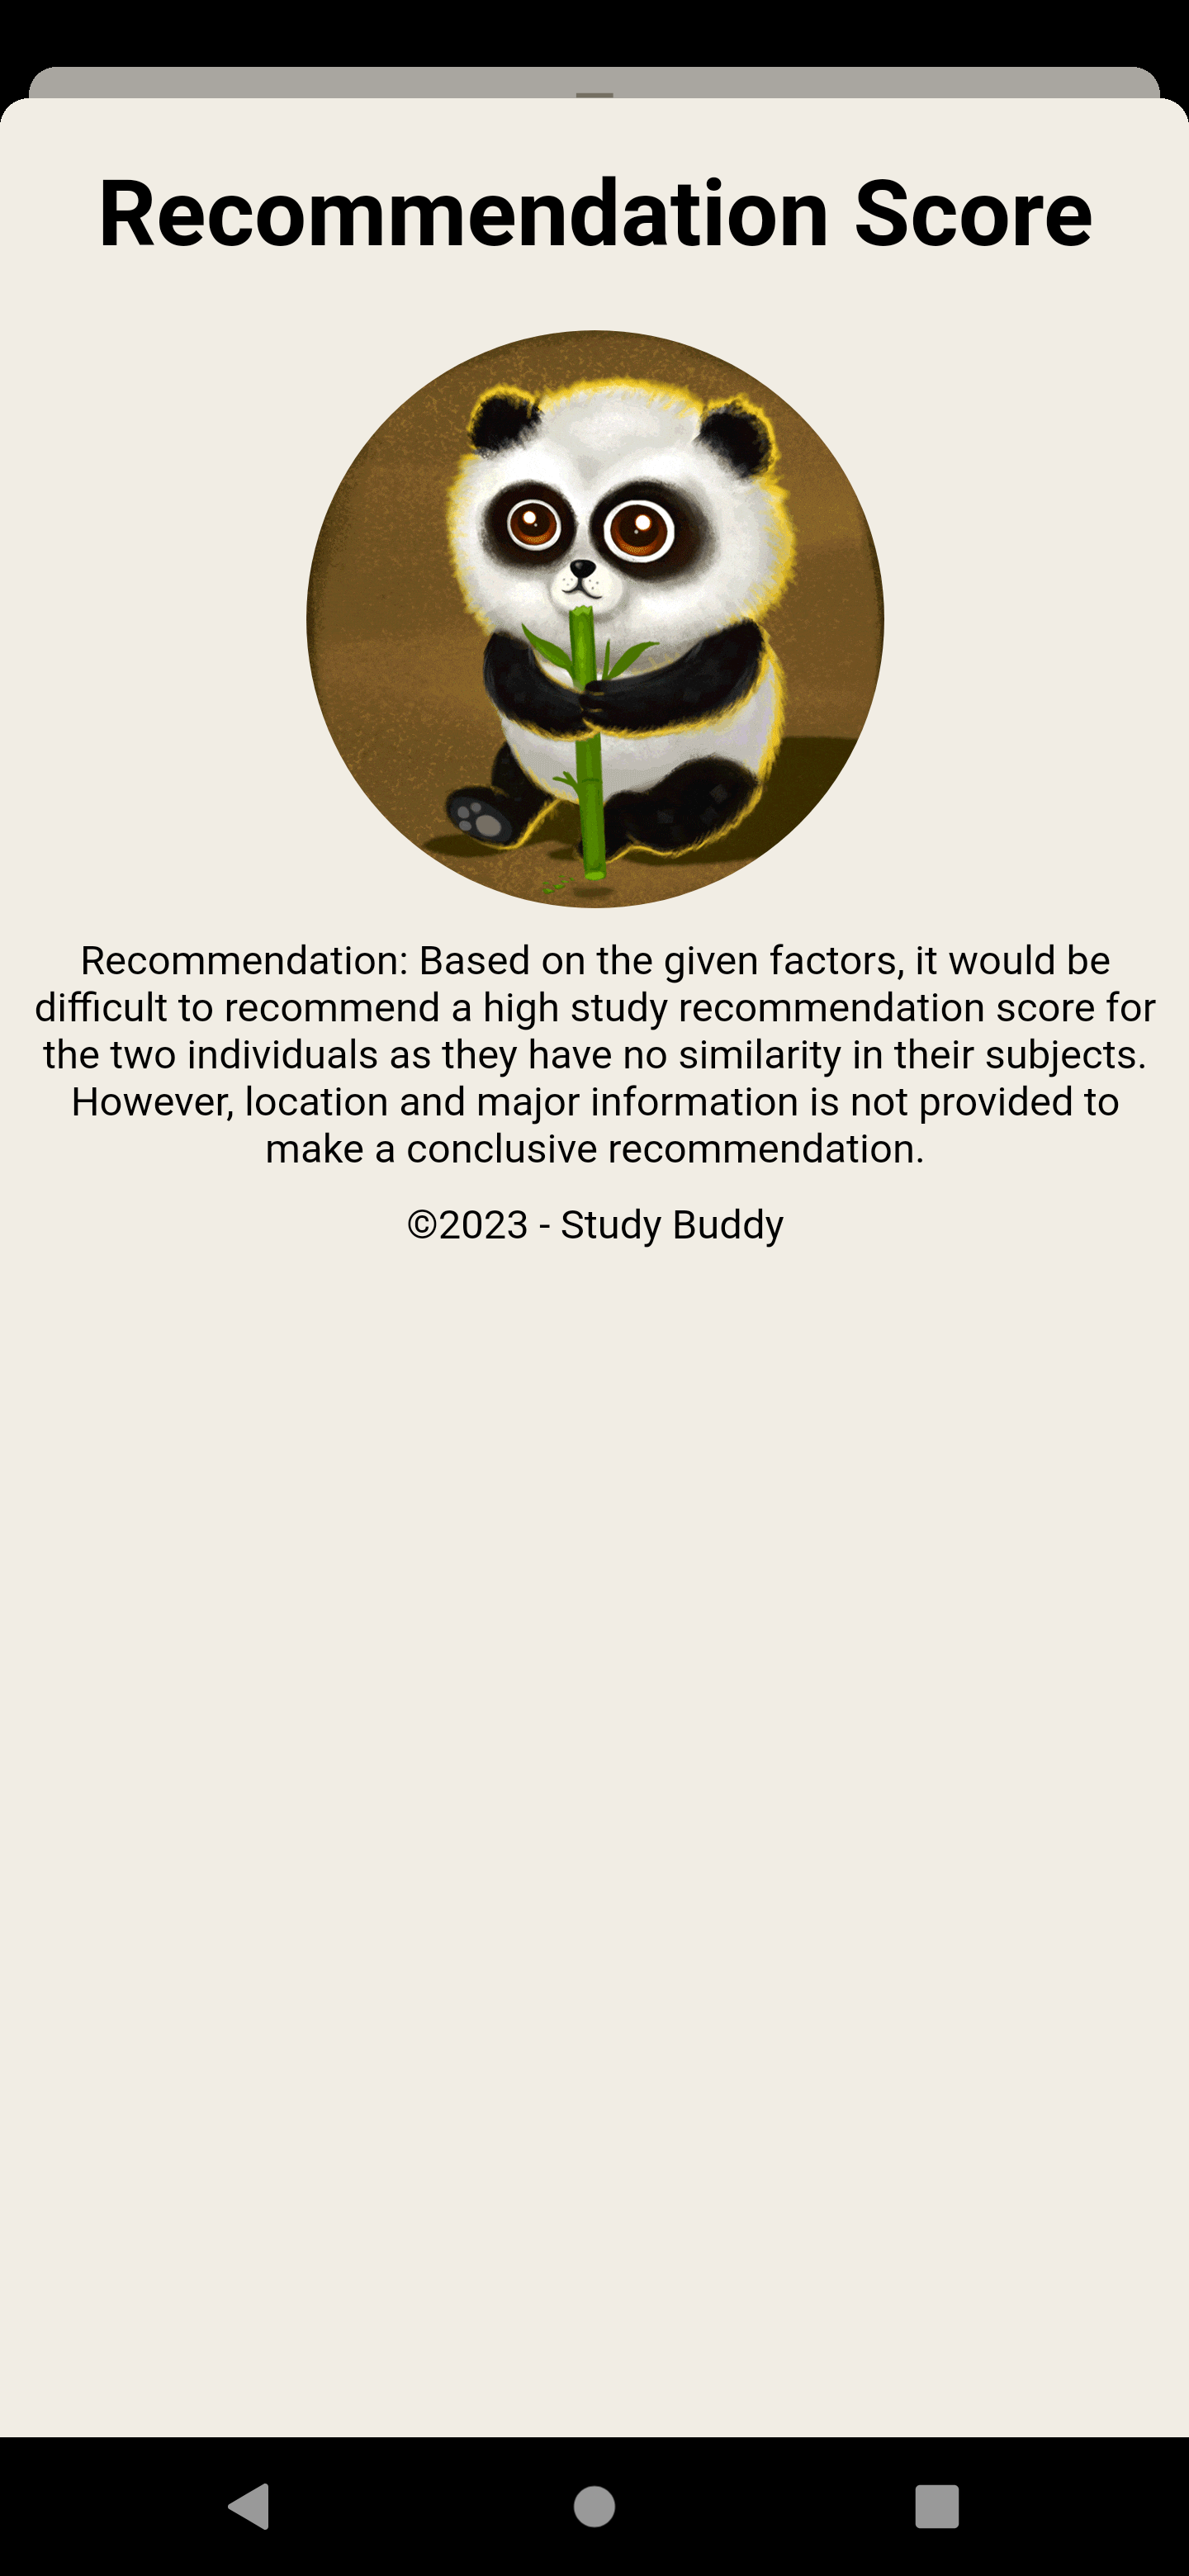
\includegraphics[width=0.45\linewidth, width=5cm, height=10cm]{images/snapshots/recommendation_score.png}}
	\hspace{5pt}
	\subcaptionbox{Error}{
		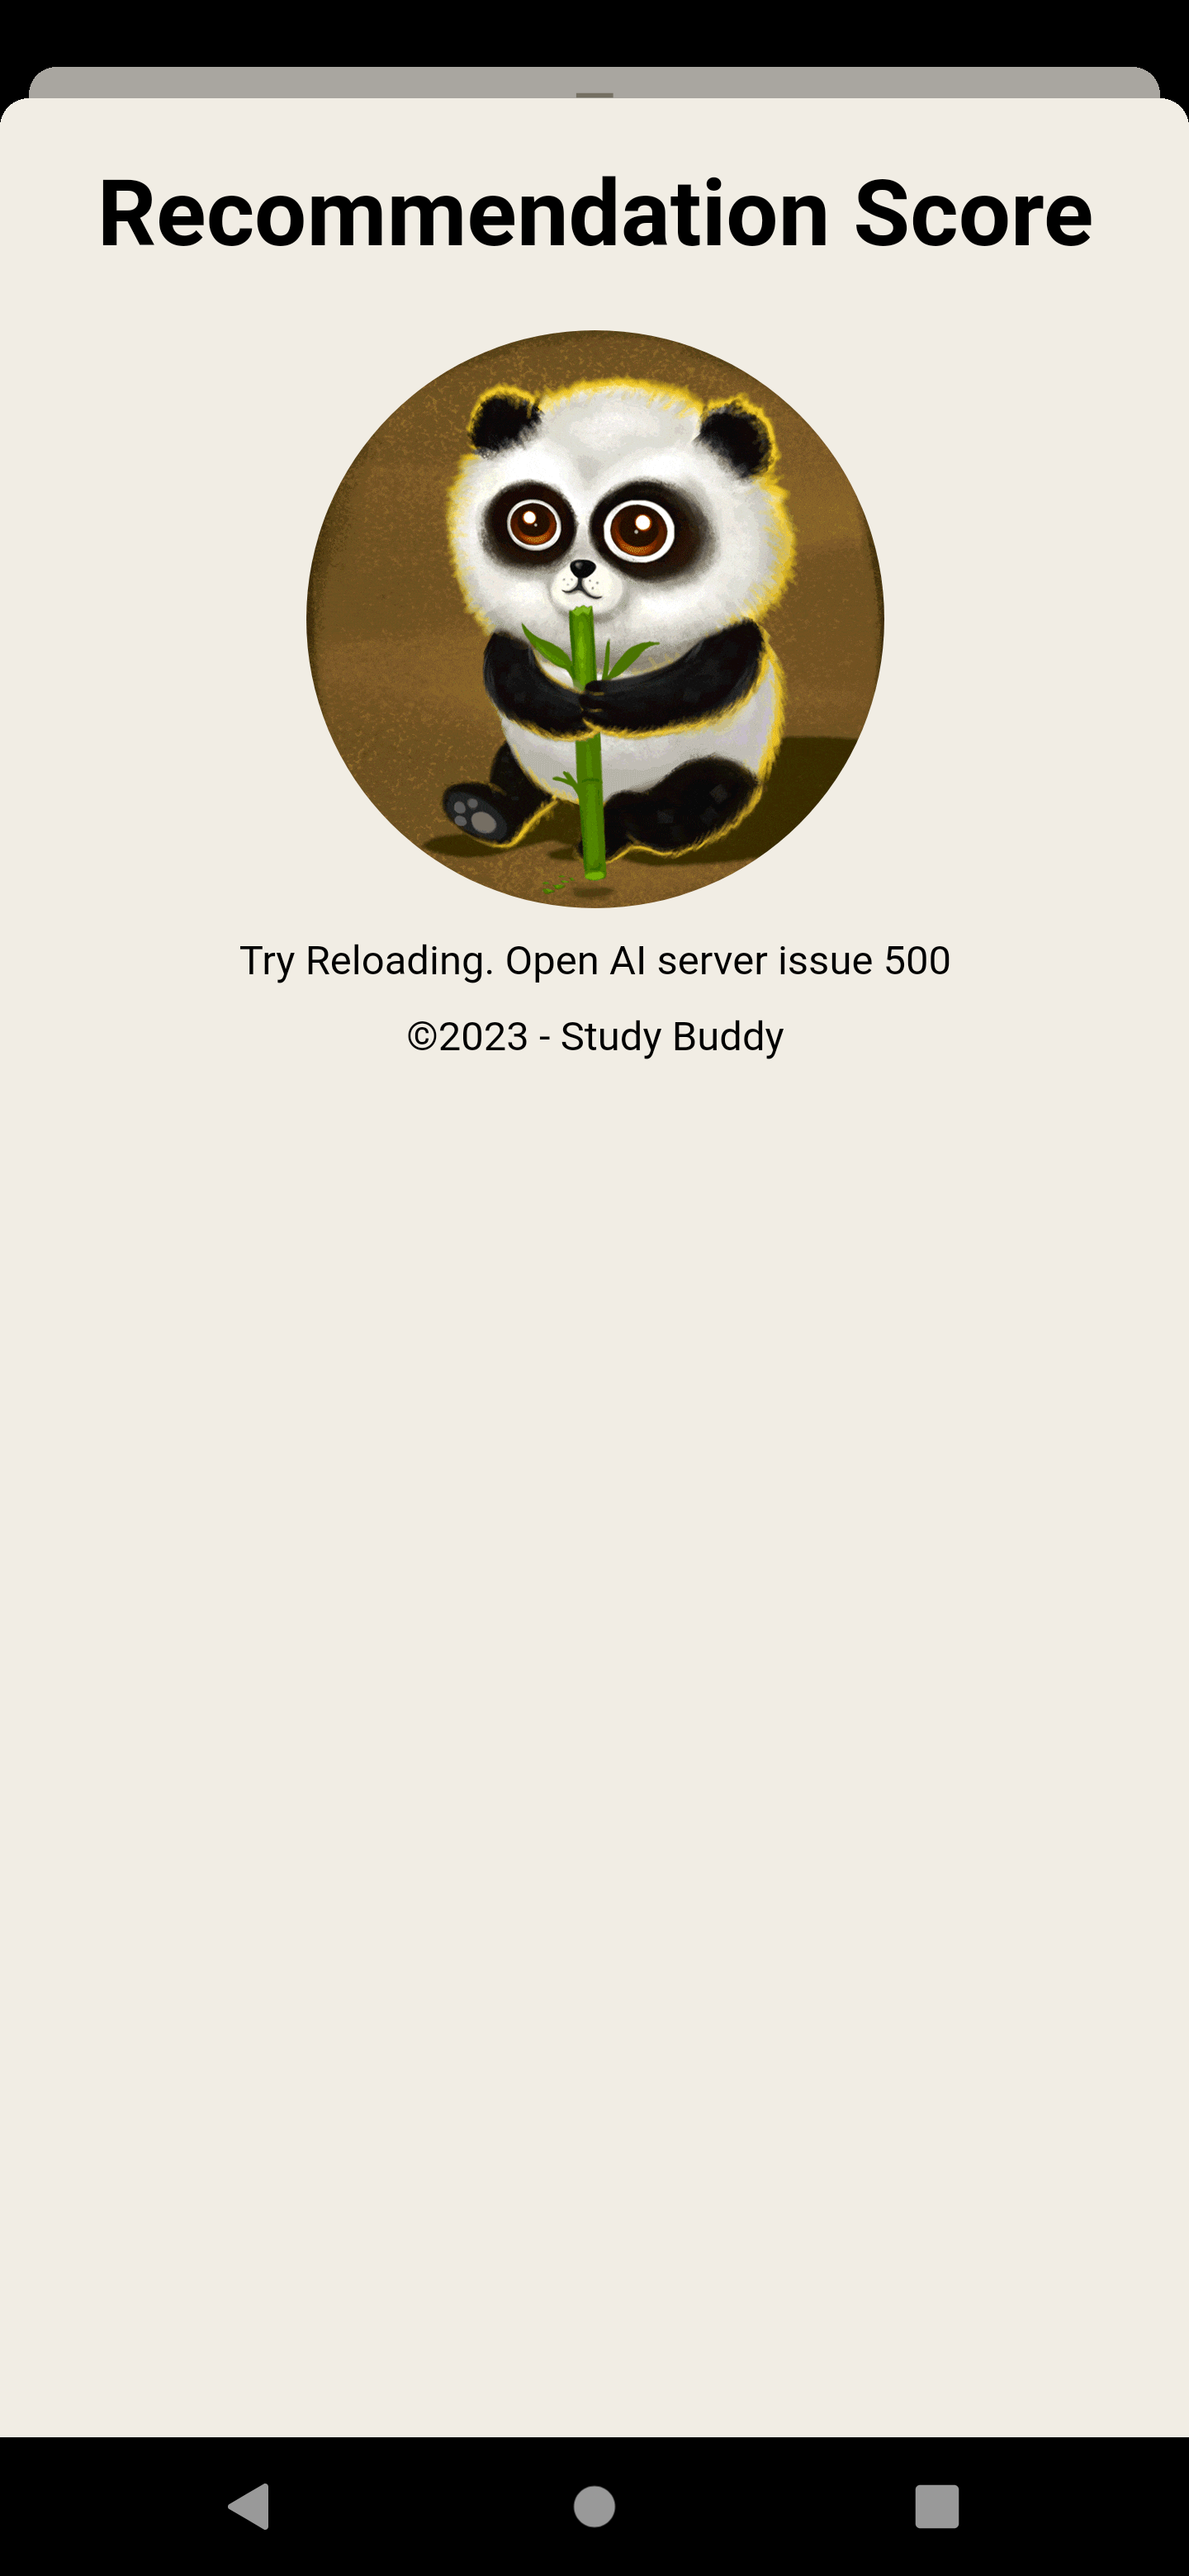
\includegraphics[width=0.45\linewidth, width=5cm, height=10cm]{images/snapshots/score_error.png}}
	\caption{Recommendation}
	\label{fig:recommend}
\end{figure}
\subsection{Matches and Messaging}
When two users mutually swipe right on each other's cards, they are instantly connected as "buddies". The user who swipes right for the second time will be shown a Match notification screen as shown in Figure~\ref{fig:matching_messaging}. From there, they can effortlessly navigate to the messages screen and initiate a conversation with their new buddy. The messaging system operates on an asynchronous model, where messages are fetched from the server only when the chat screen is mounted or when a new message is sent. This approach optimizes resource usage by minimizing unnecessary API calls and ensures that messages are retrieved and displayed efficiently, enhancing the overall user experience.
  \begin{figure}[H]
	\centering
	\subcaptionbox{Match Modal Notification}{
		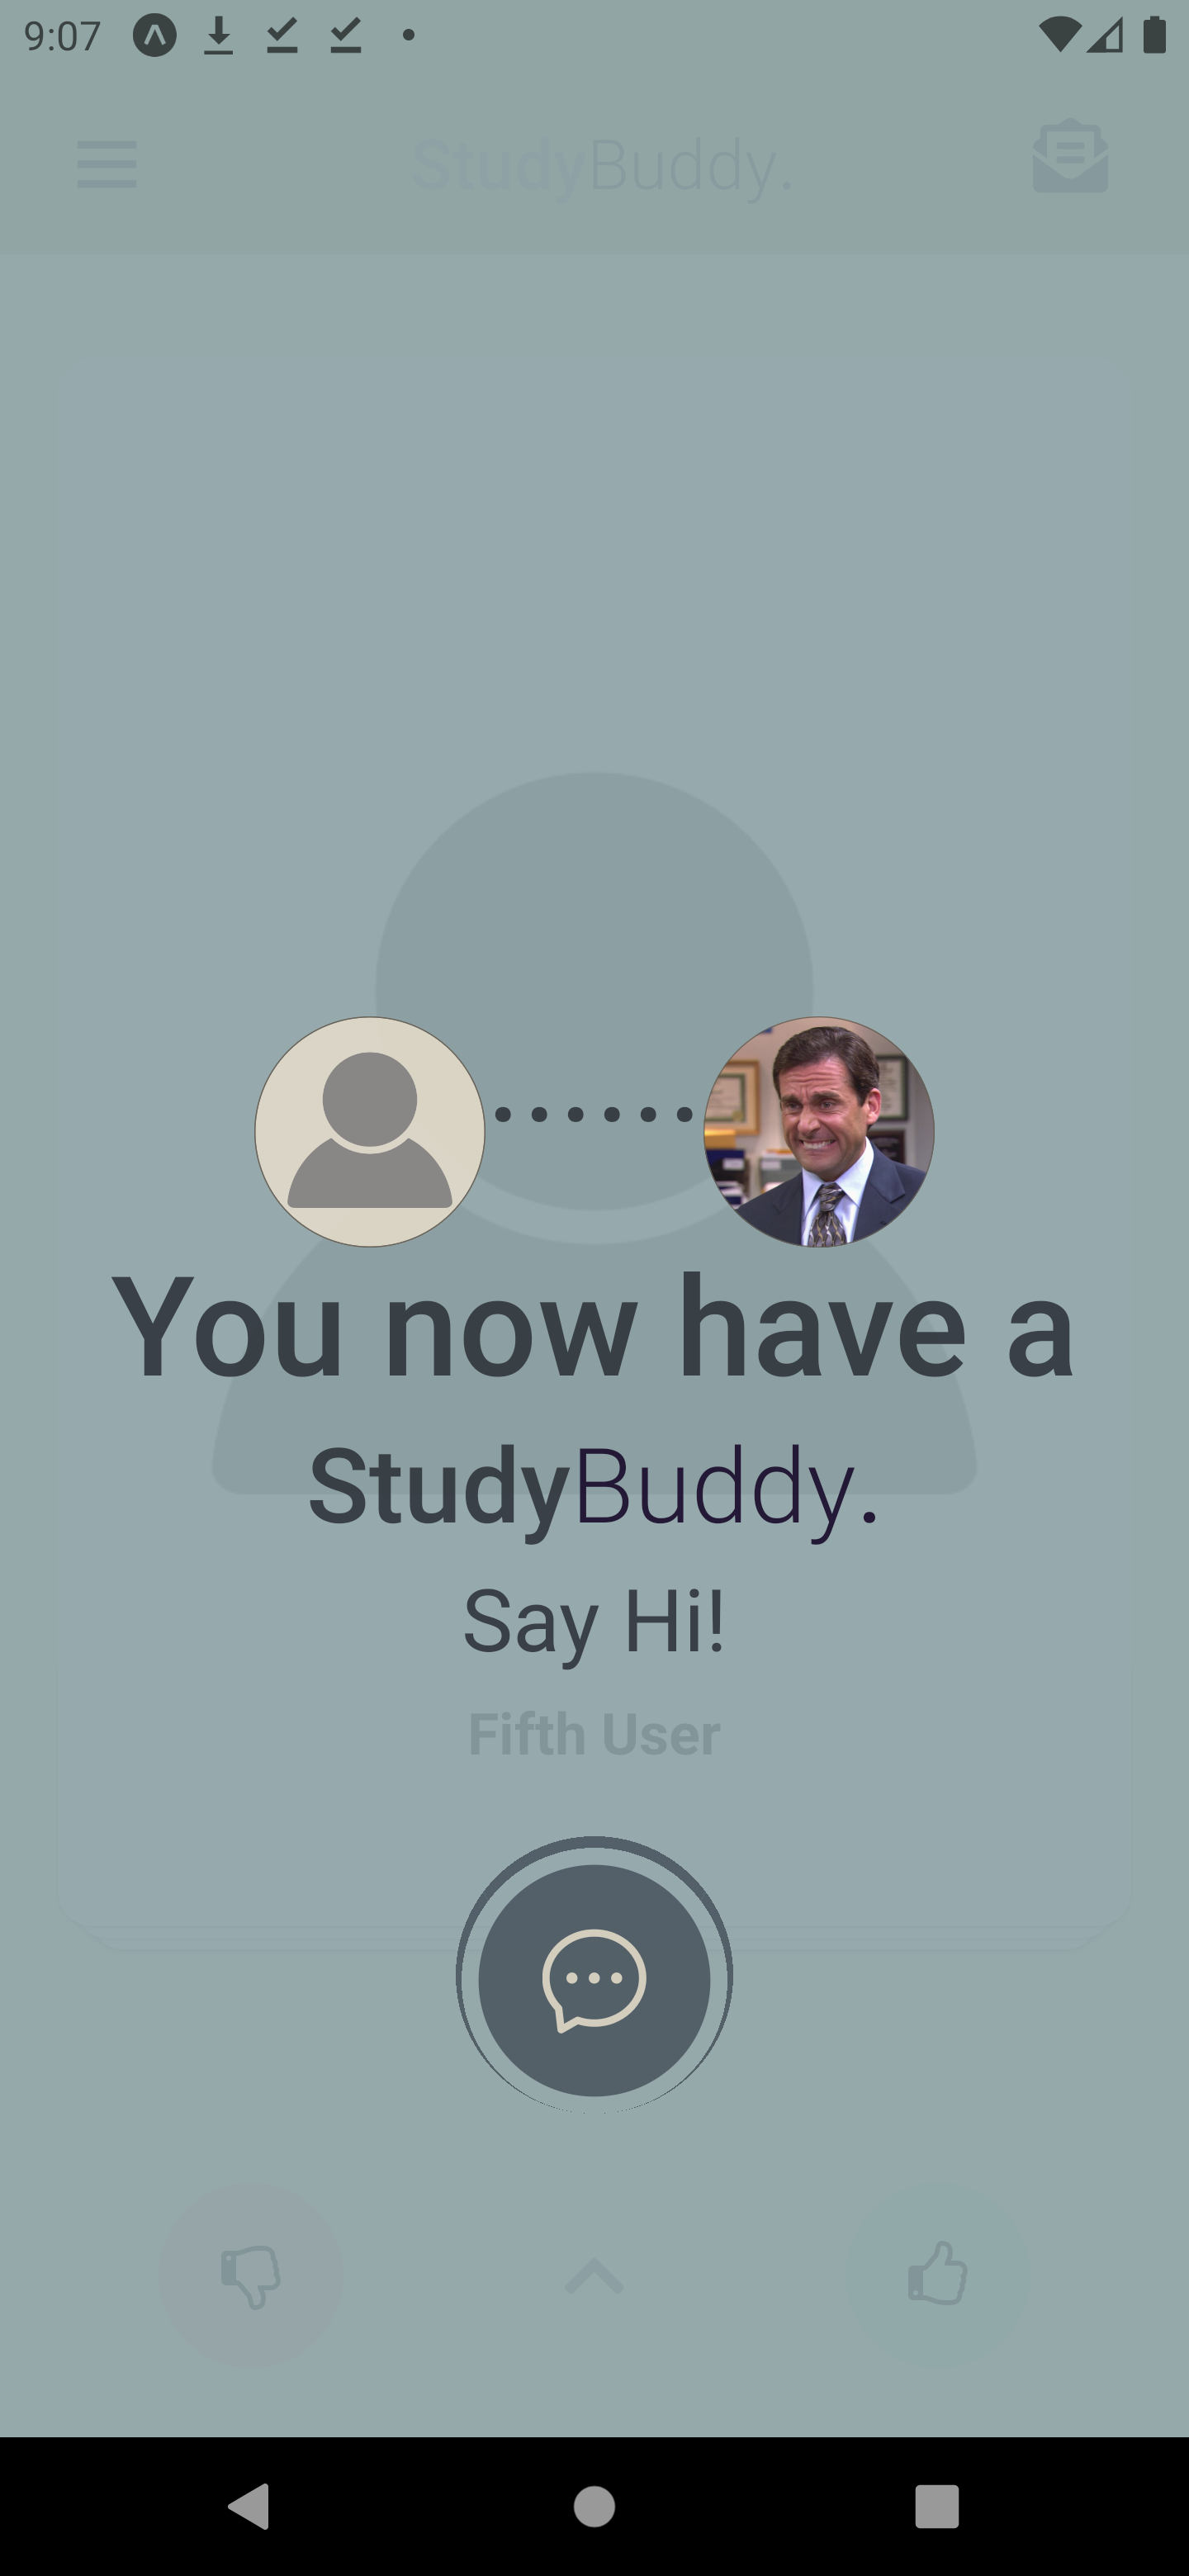
\includegraphics[width=0.45\linewidth, width=5cm, height=10cm]{images/snapshots/match_modal_screen.png}}
	\hspace{5pt}
	\subcaptionbox{Messages Screen}{
		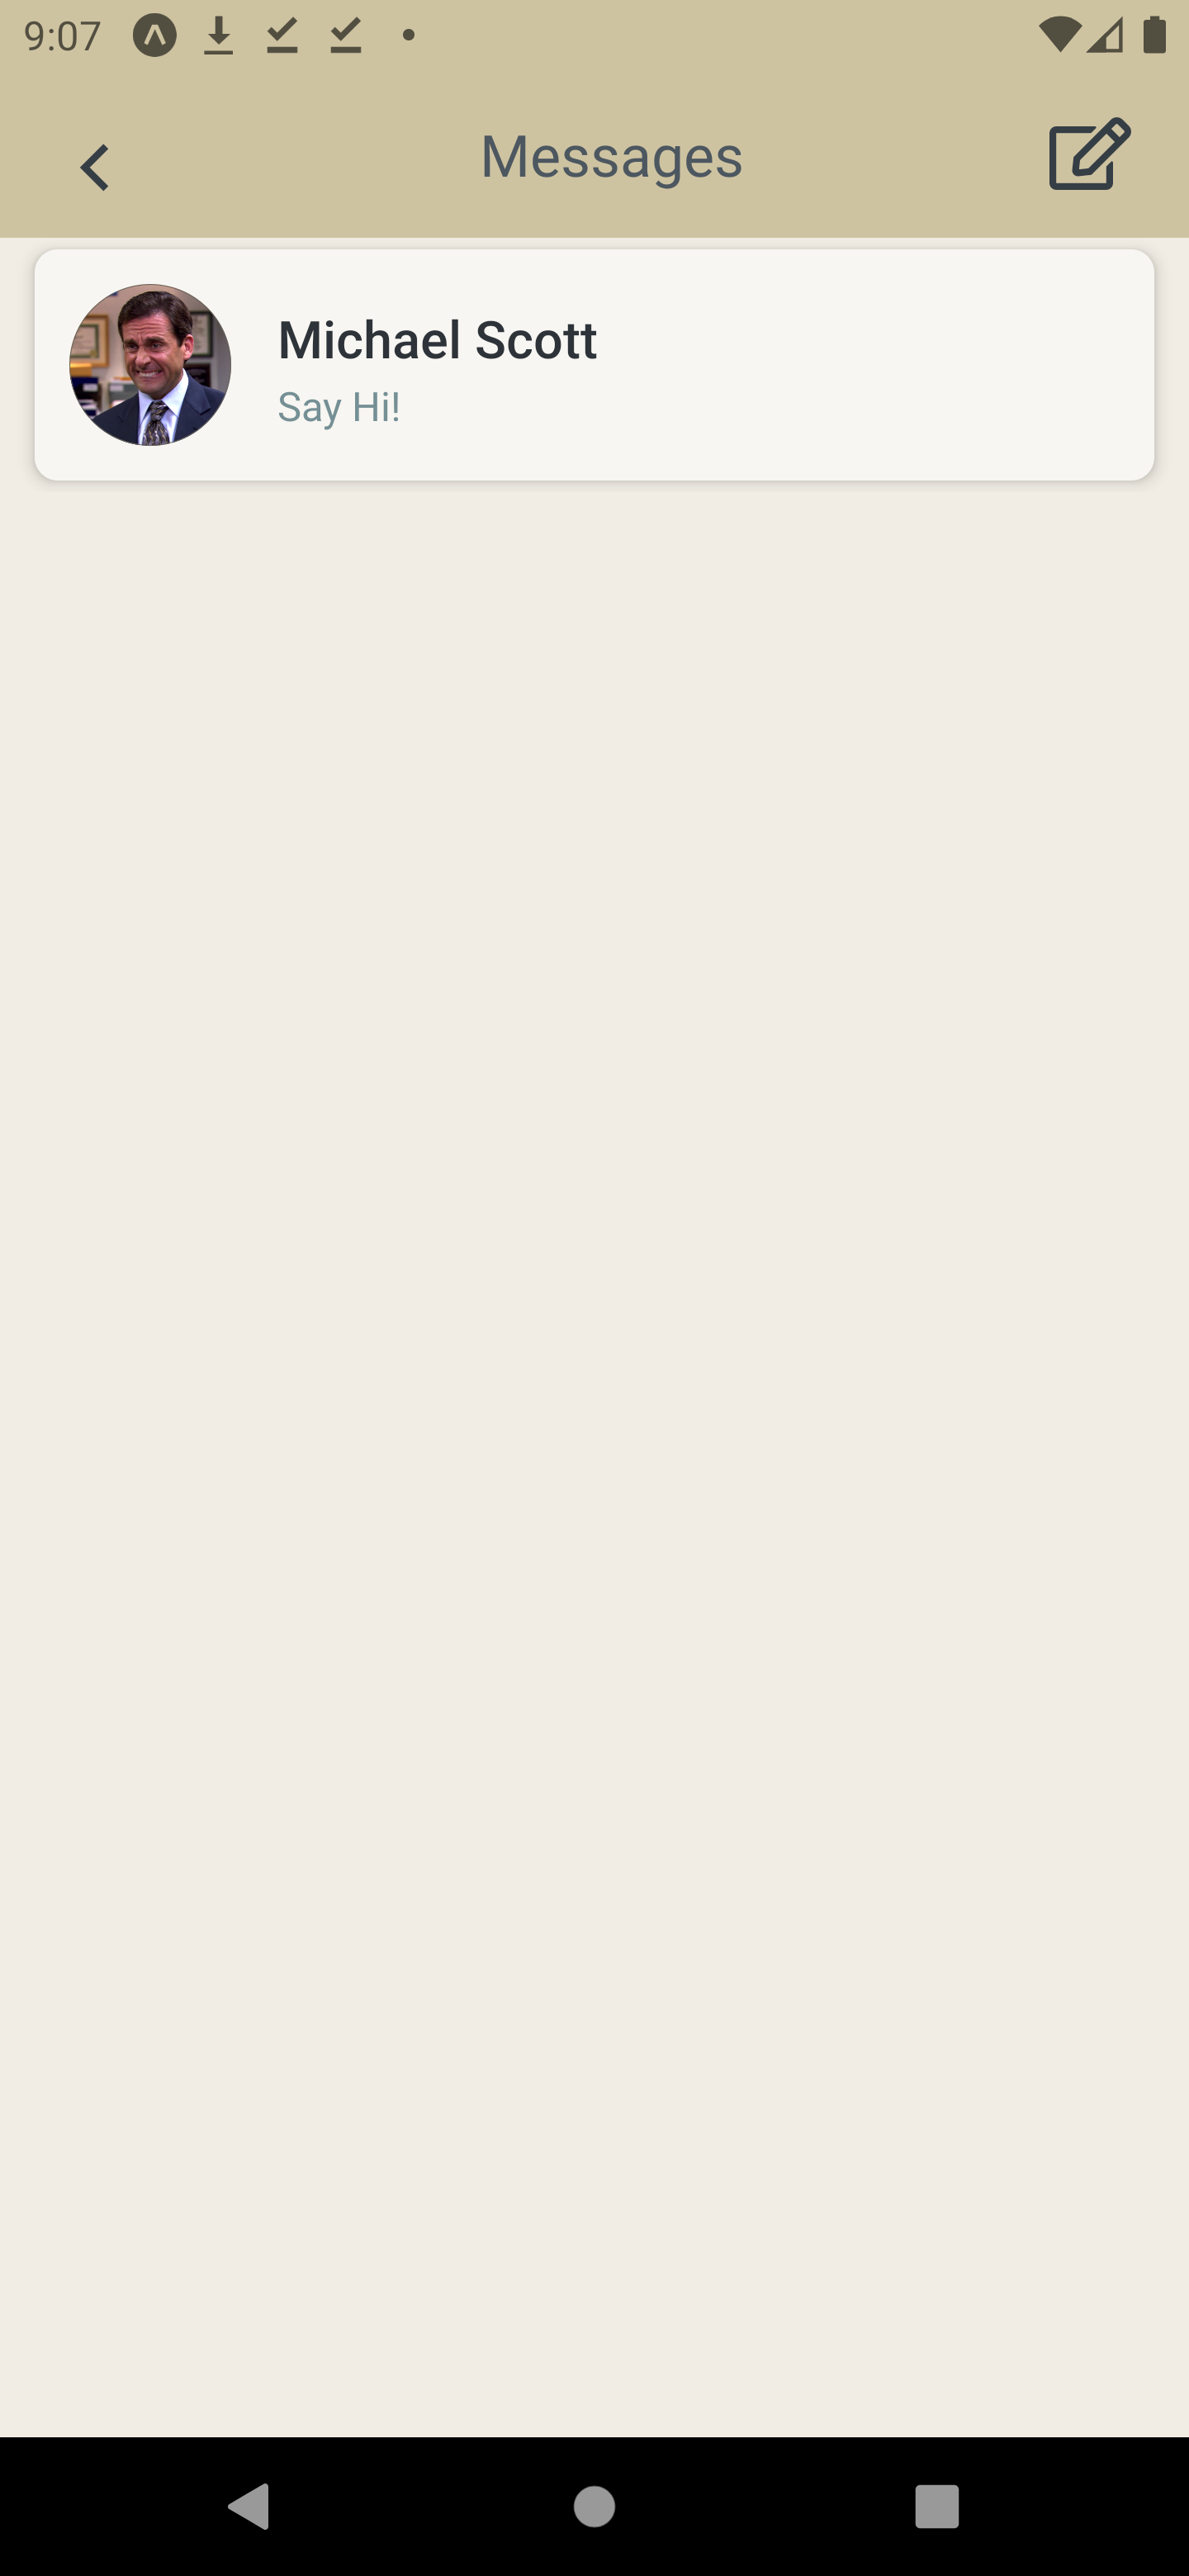
\includegraphics[width=0.45\linewidth, width=5cm, height=10cm]{images/snapshots/messages_screen.png}}
        \hspace{5pt}
	\subcaptionbox{Messages Screen}{
		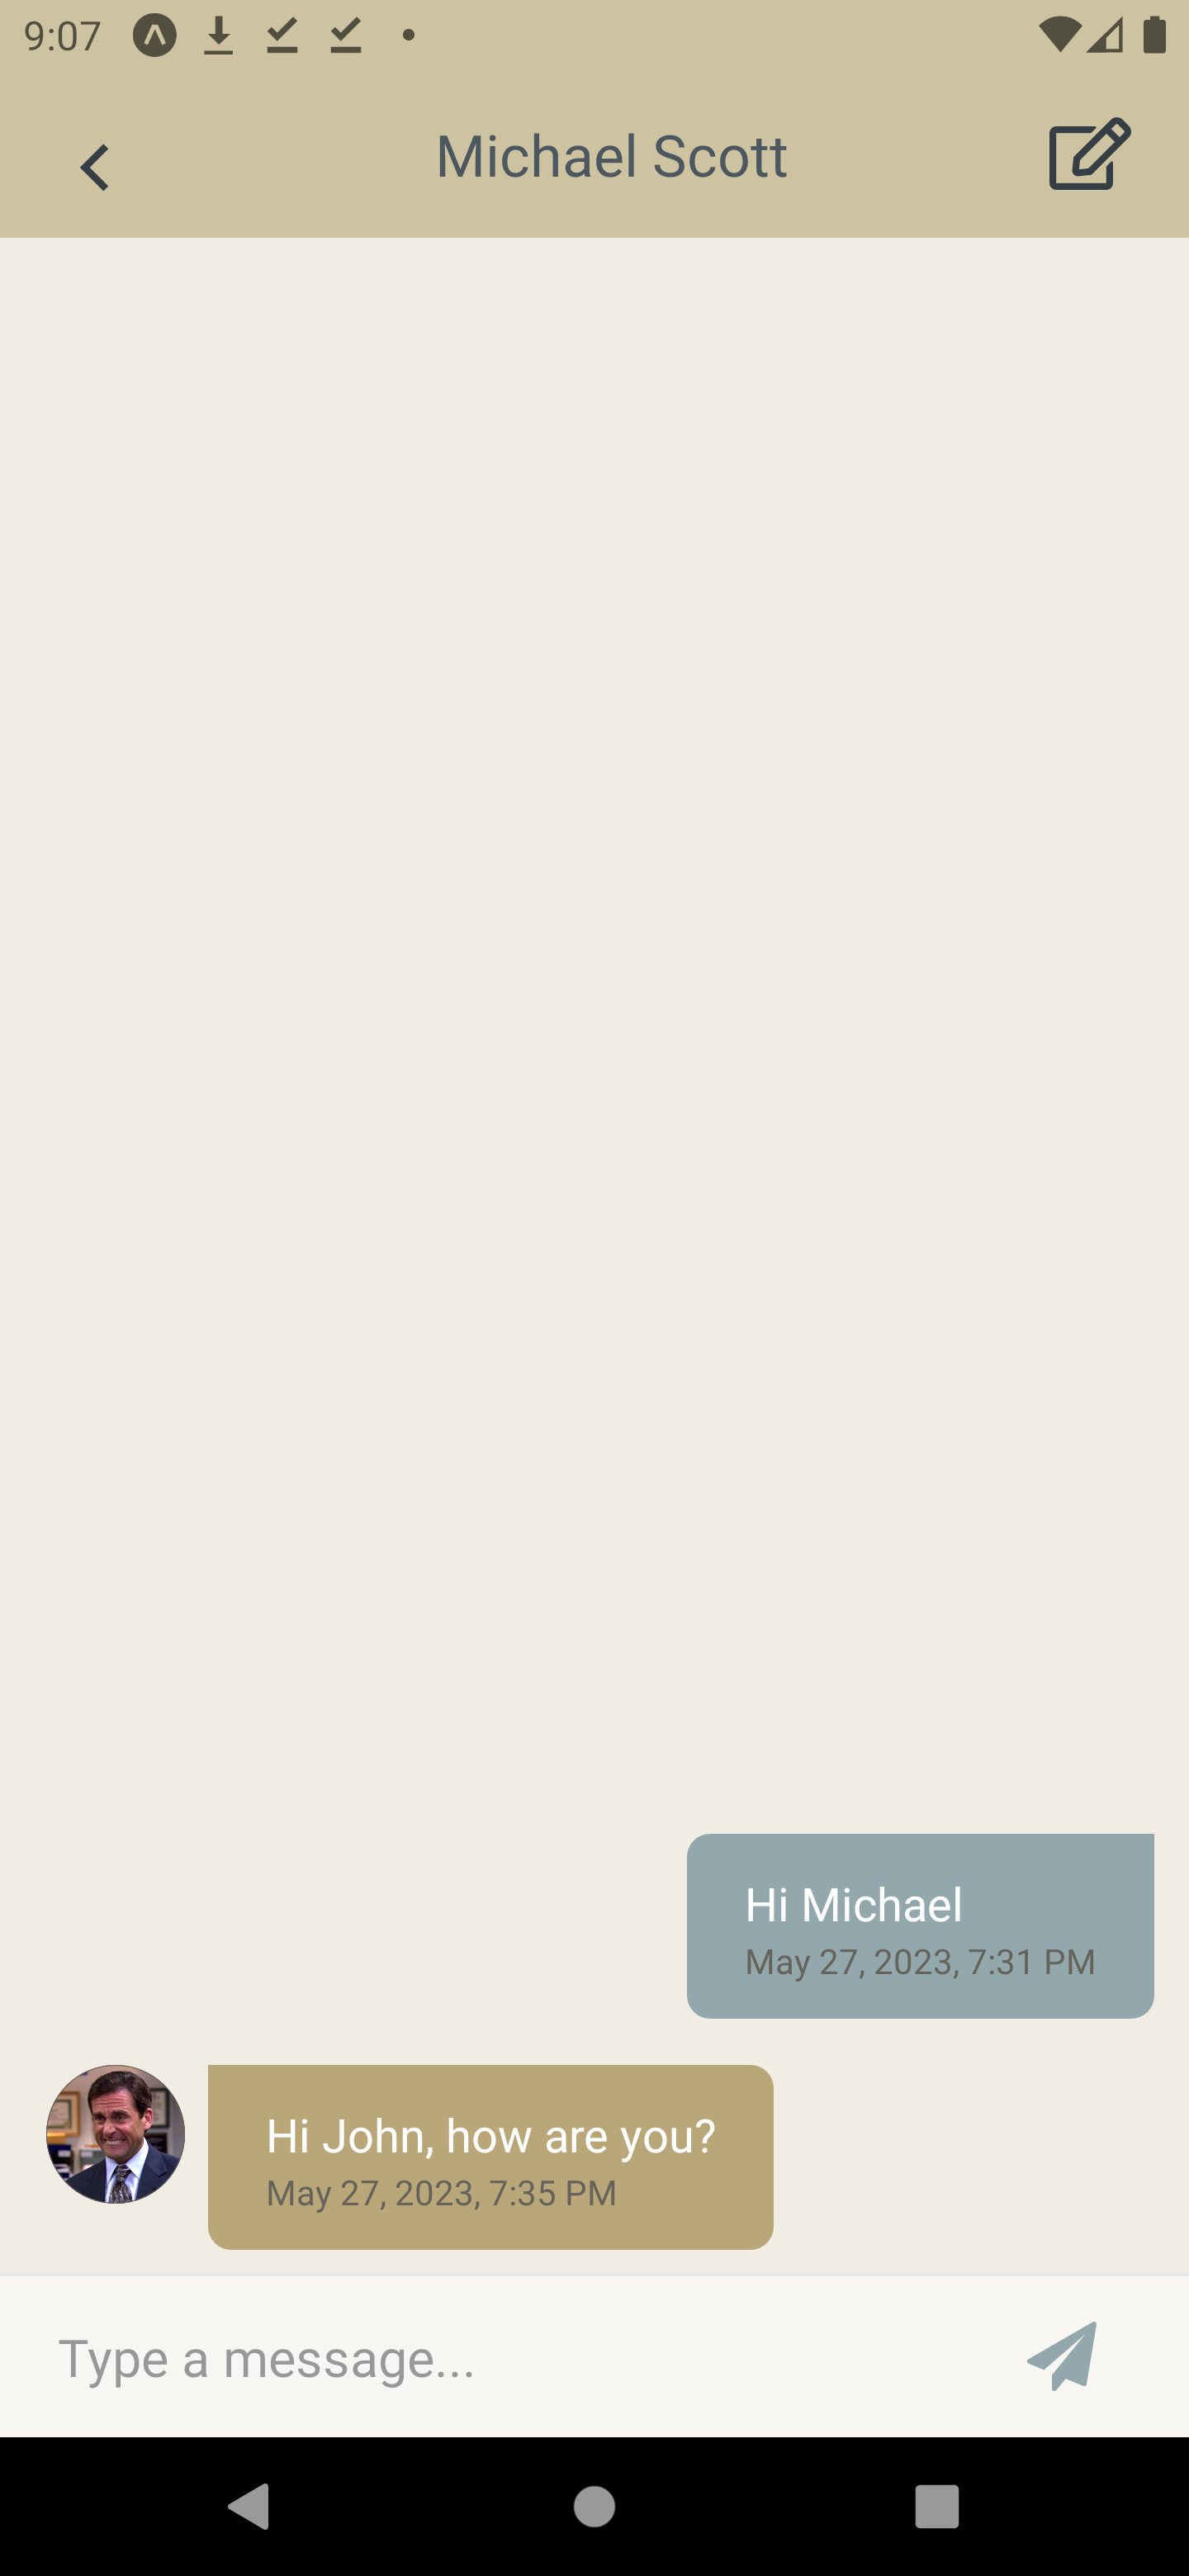
\includegraphics[width=0.45\linewidth, width=5cm, height=10cm]{images/snapshots/chat_screen_2.png}}
	\caption{Matching}
	\label{fig:matching_messaging}
\end{figure}
\subsection{Navigation Options}
The home screen provides several navigation options as shown in Figure~\ref{fig:drawer}. A header with a messages icon allows users to access the messages screen from anywhere in the app. The top-left corner features a navicon that opens a drawer, which can also be accessed by sliding right on the screen. The drawer displays the logged-in user's profile image and number of buddies. Navigational options within the drawer include Home screen, Edit Profile screen, Matches screen, Contact Us screen, and Logout button.
  \begin{figure}[H]
	\centering
	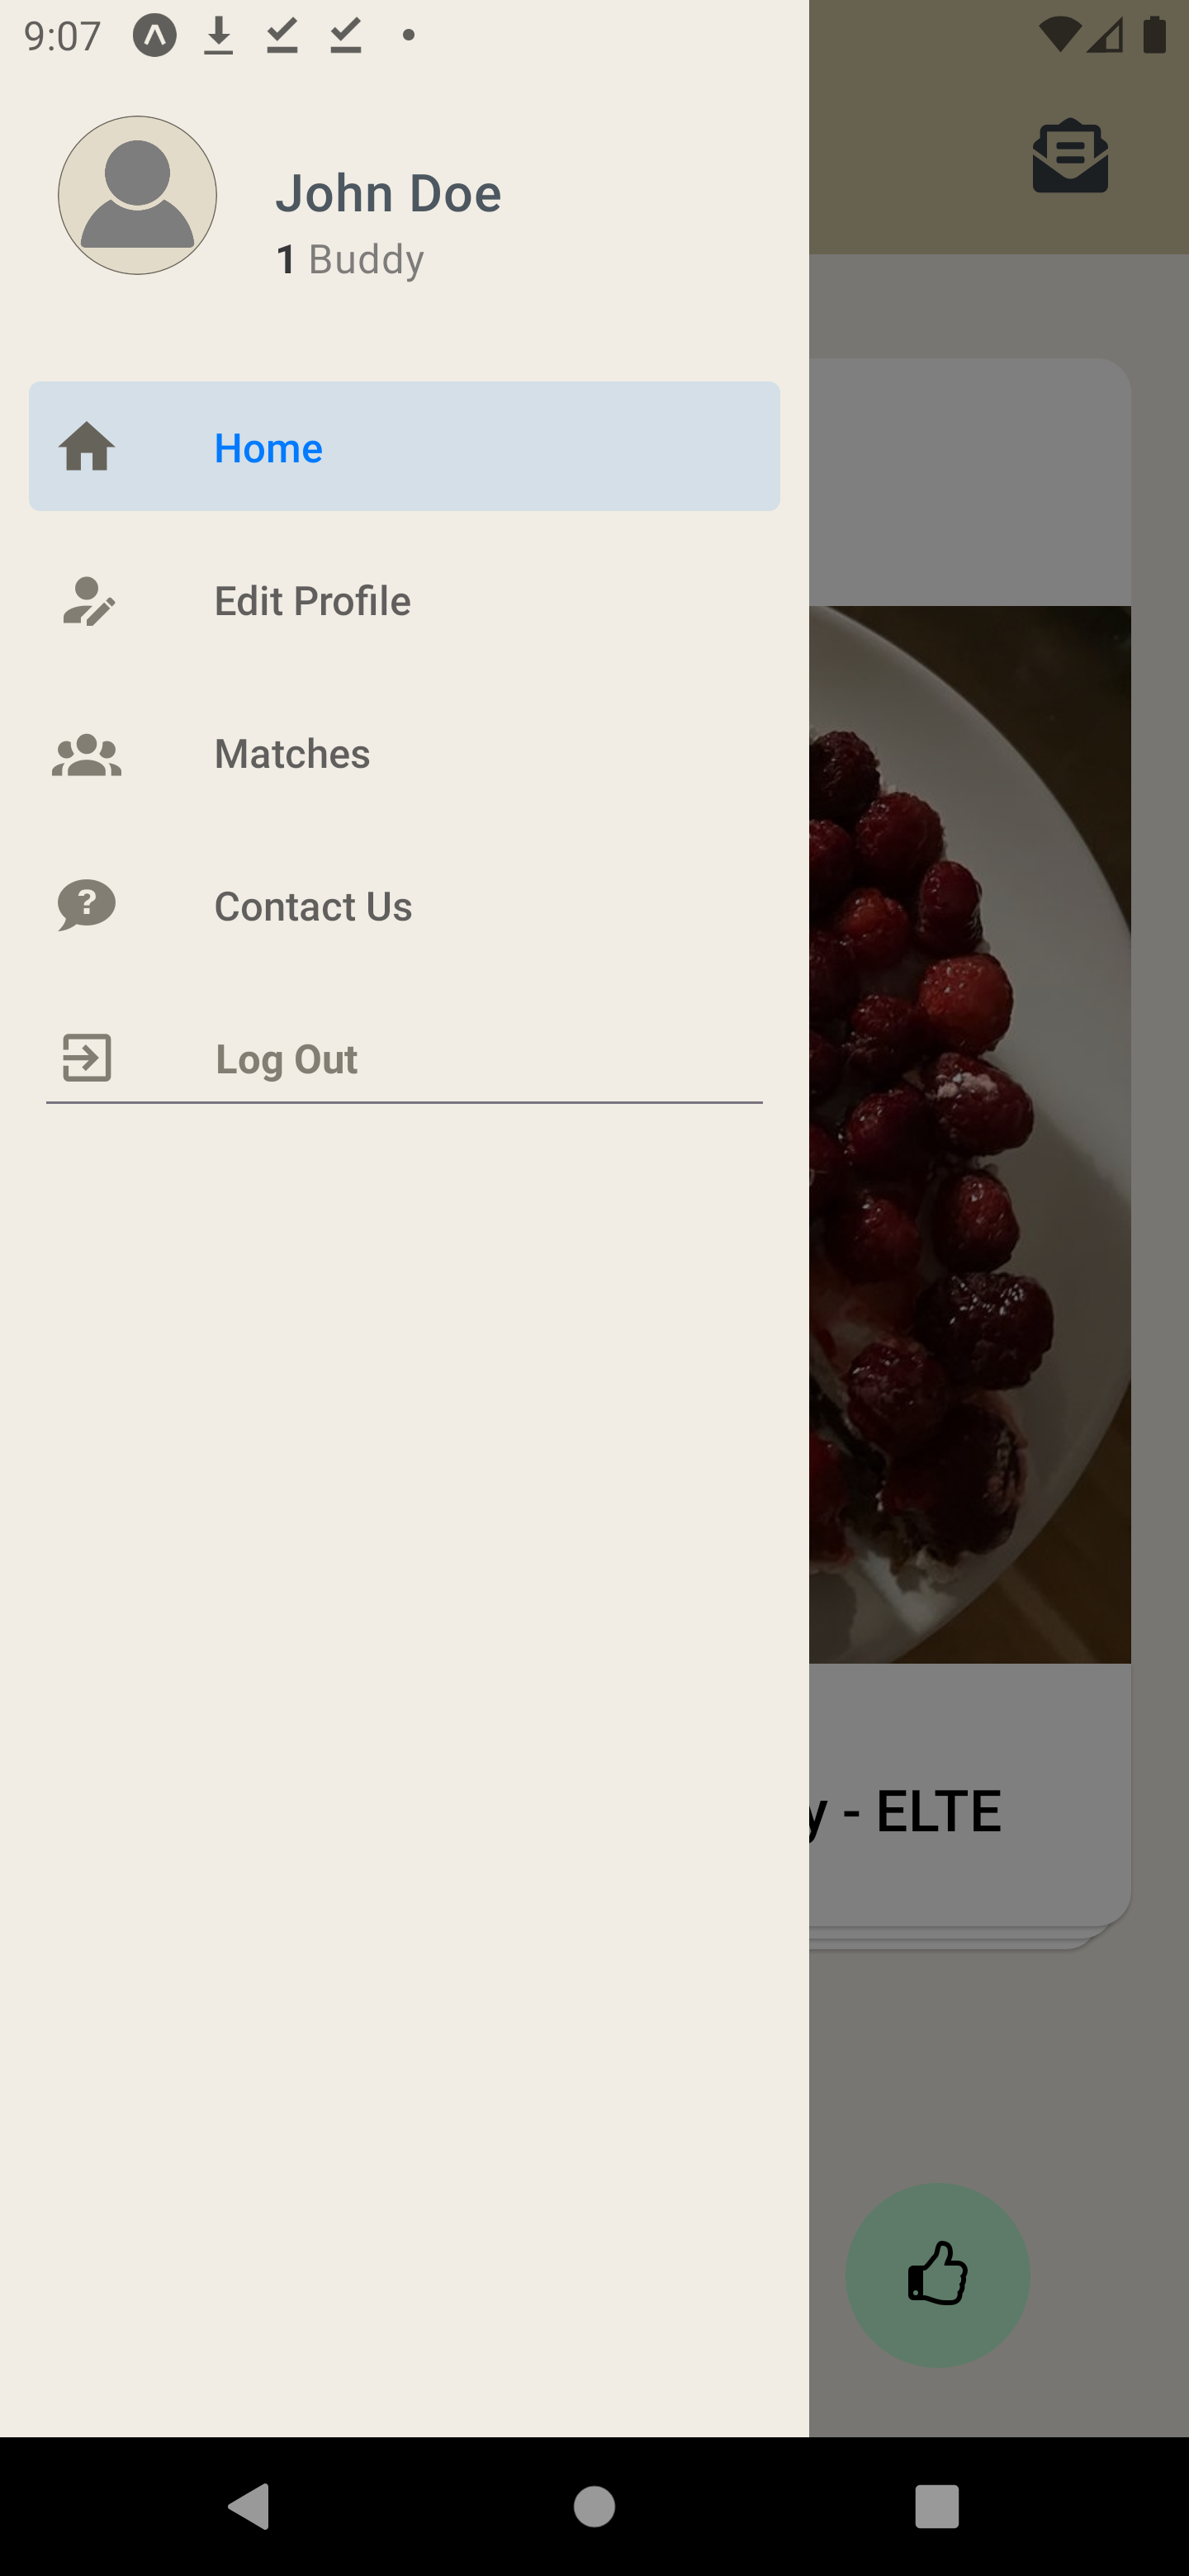
\includegraphics[width=0.45\linewidth, width=5cm, height=10cm]{images/snapshots/logout.png}
        \caption{Drawer}
	\label{fig:drawer}
  \end{figure}
\subsection{Edit Profile}
On this screen, users can make changes to their profile picture, bio, age, and other mandatory information. To update the profile, users have to scroll to the bottom and click the update profile button. They can also delete their accounts here if needed as shown in the Figure~\ref{fig:edit-profile-screen}.
   \begin{figure}[H]
	\centering
	\subcaptionbox{Edit}{
		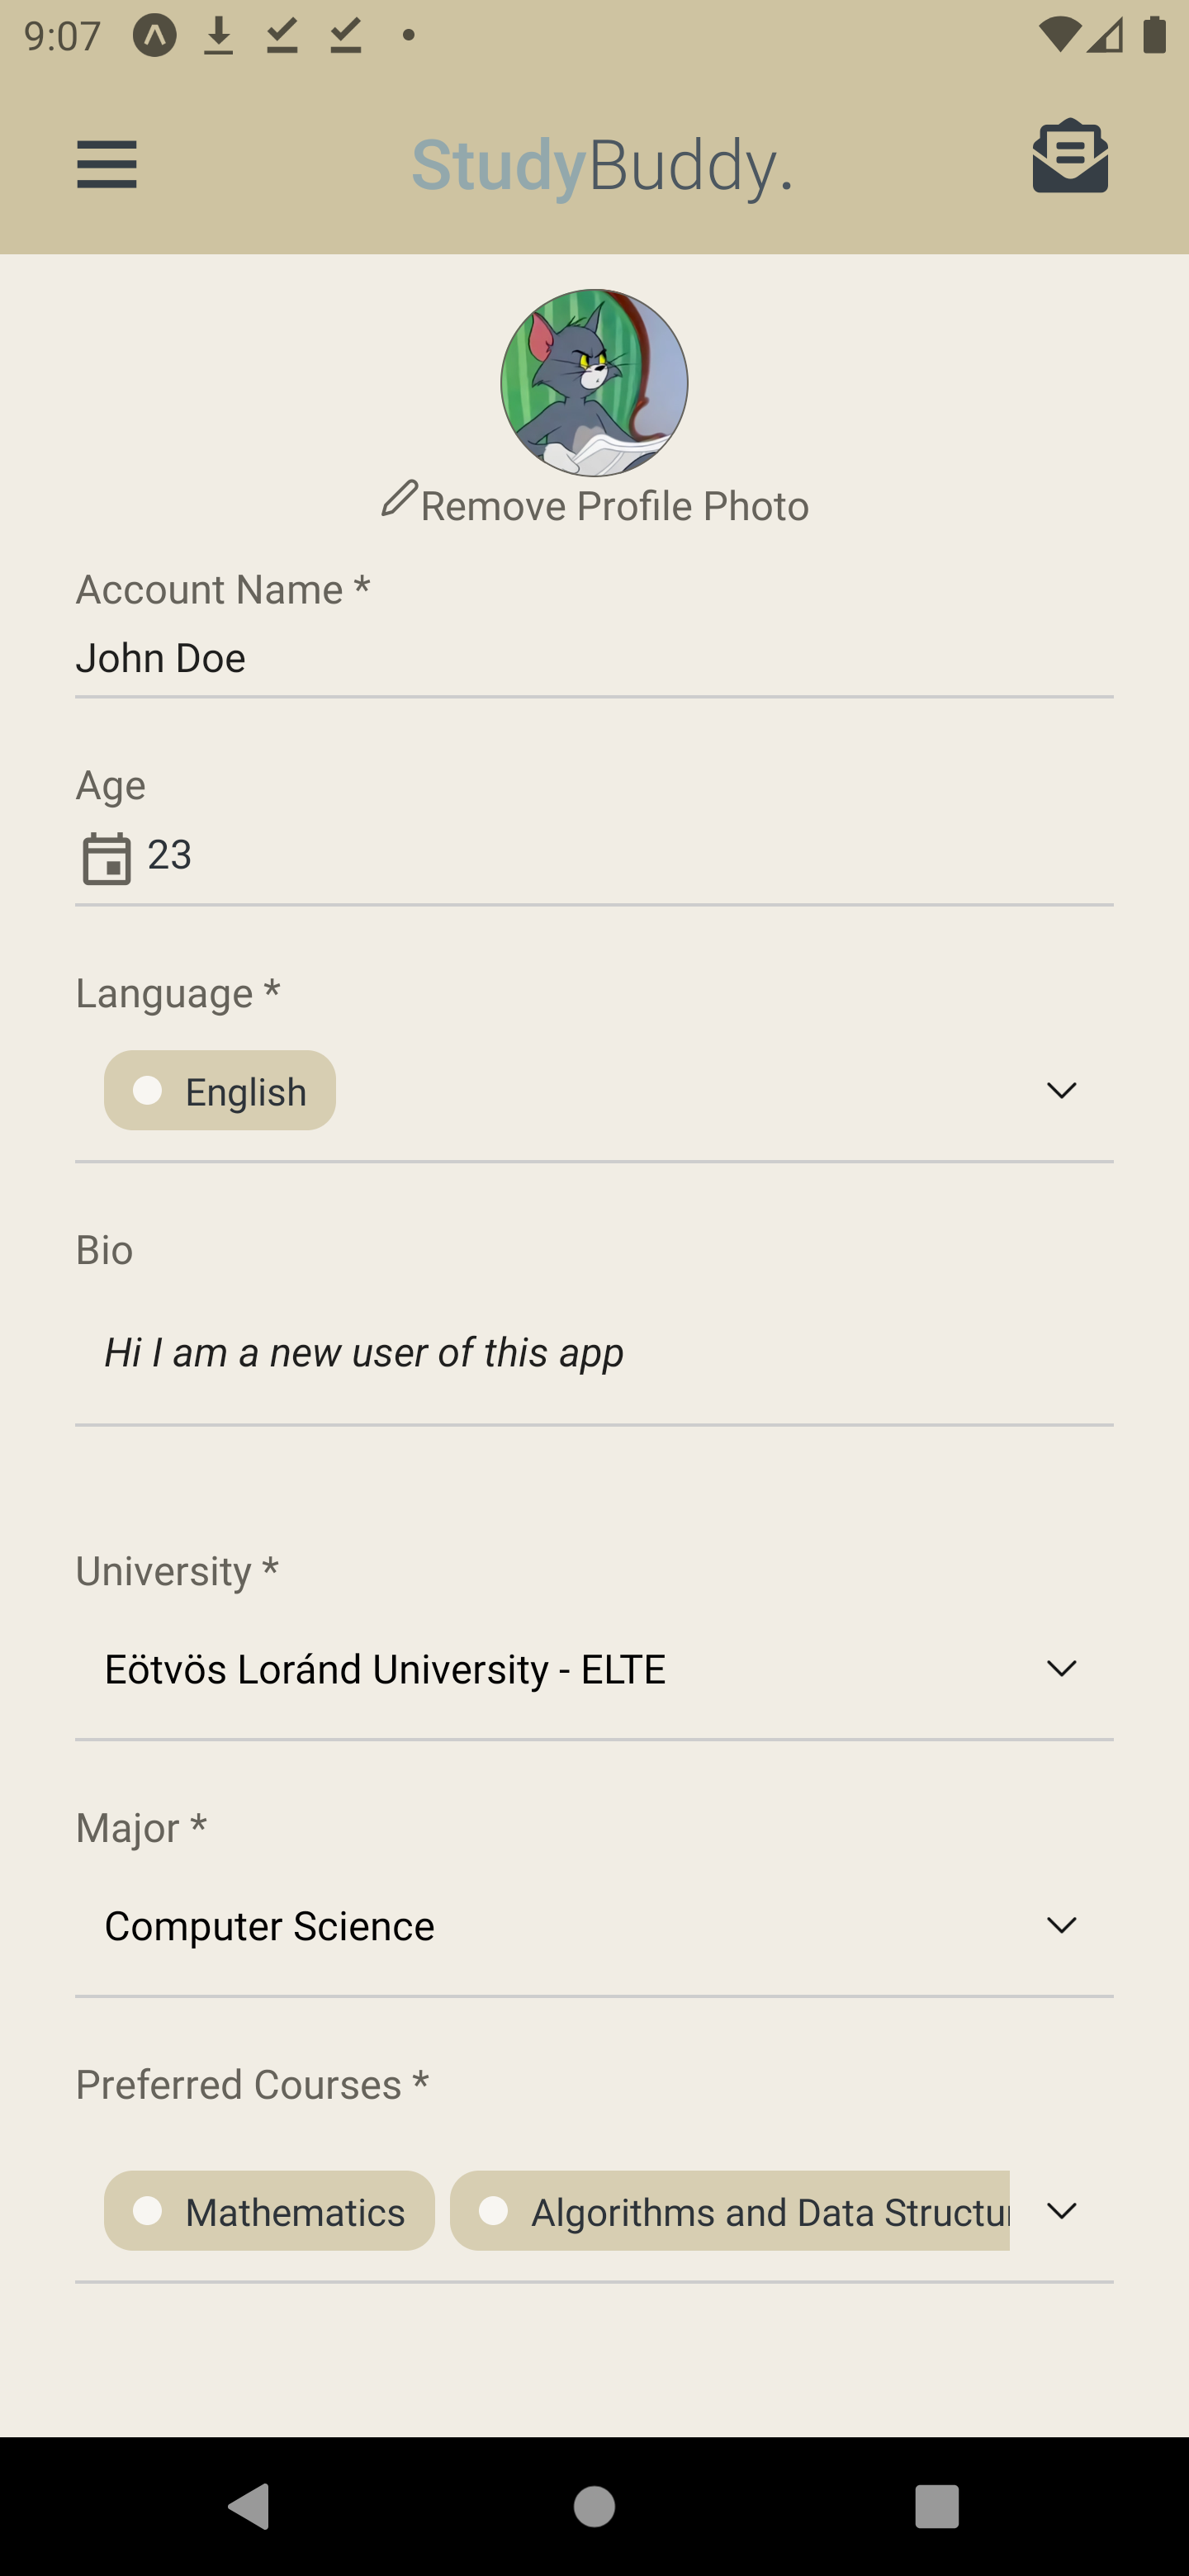
\includegraphics[width=0.45\linewidth, width=5cm, height=10cm]{images/snapshots/edit_profile_1.png}}
	\hspace{5pt}
	\subcaptionbox{Update}{
		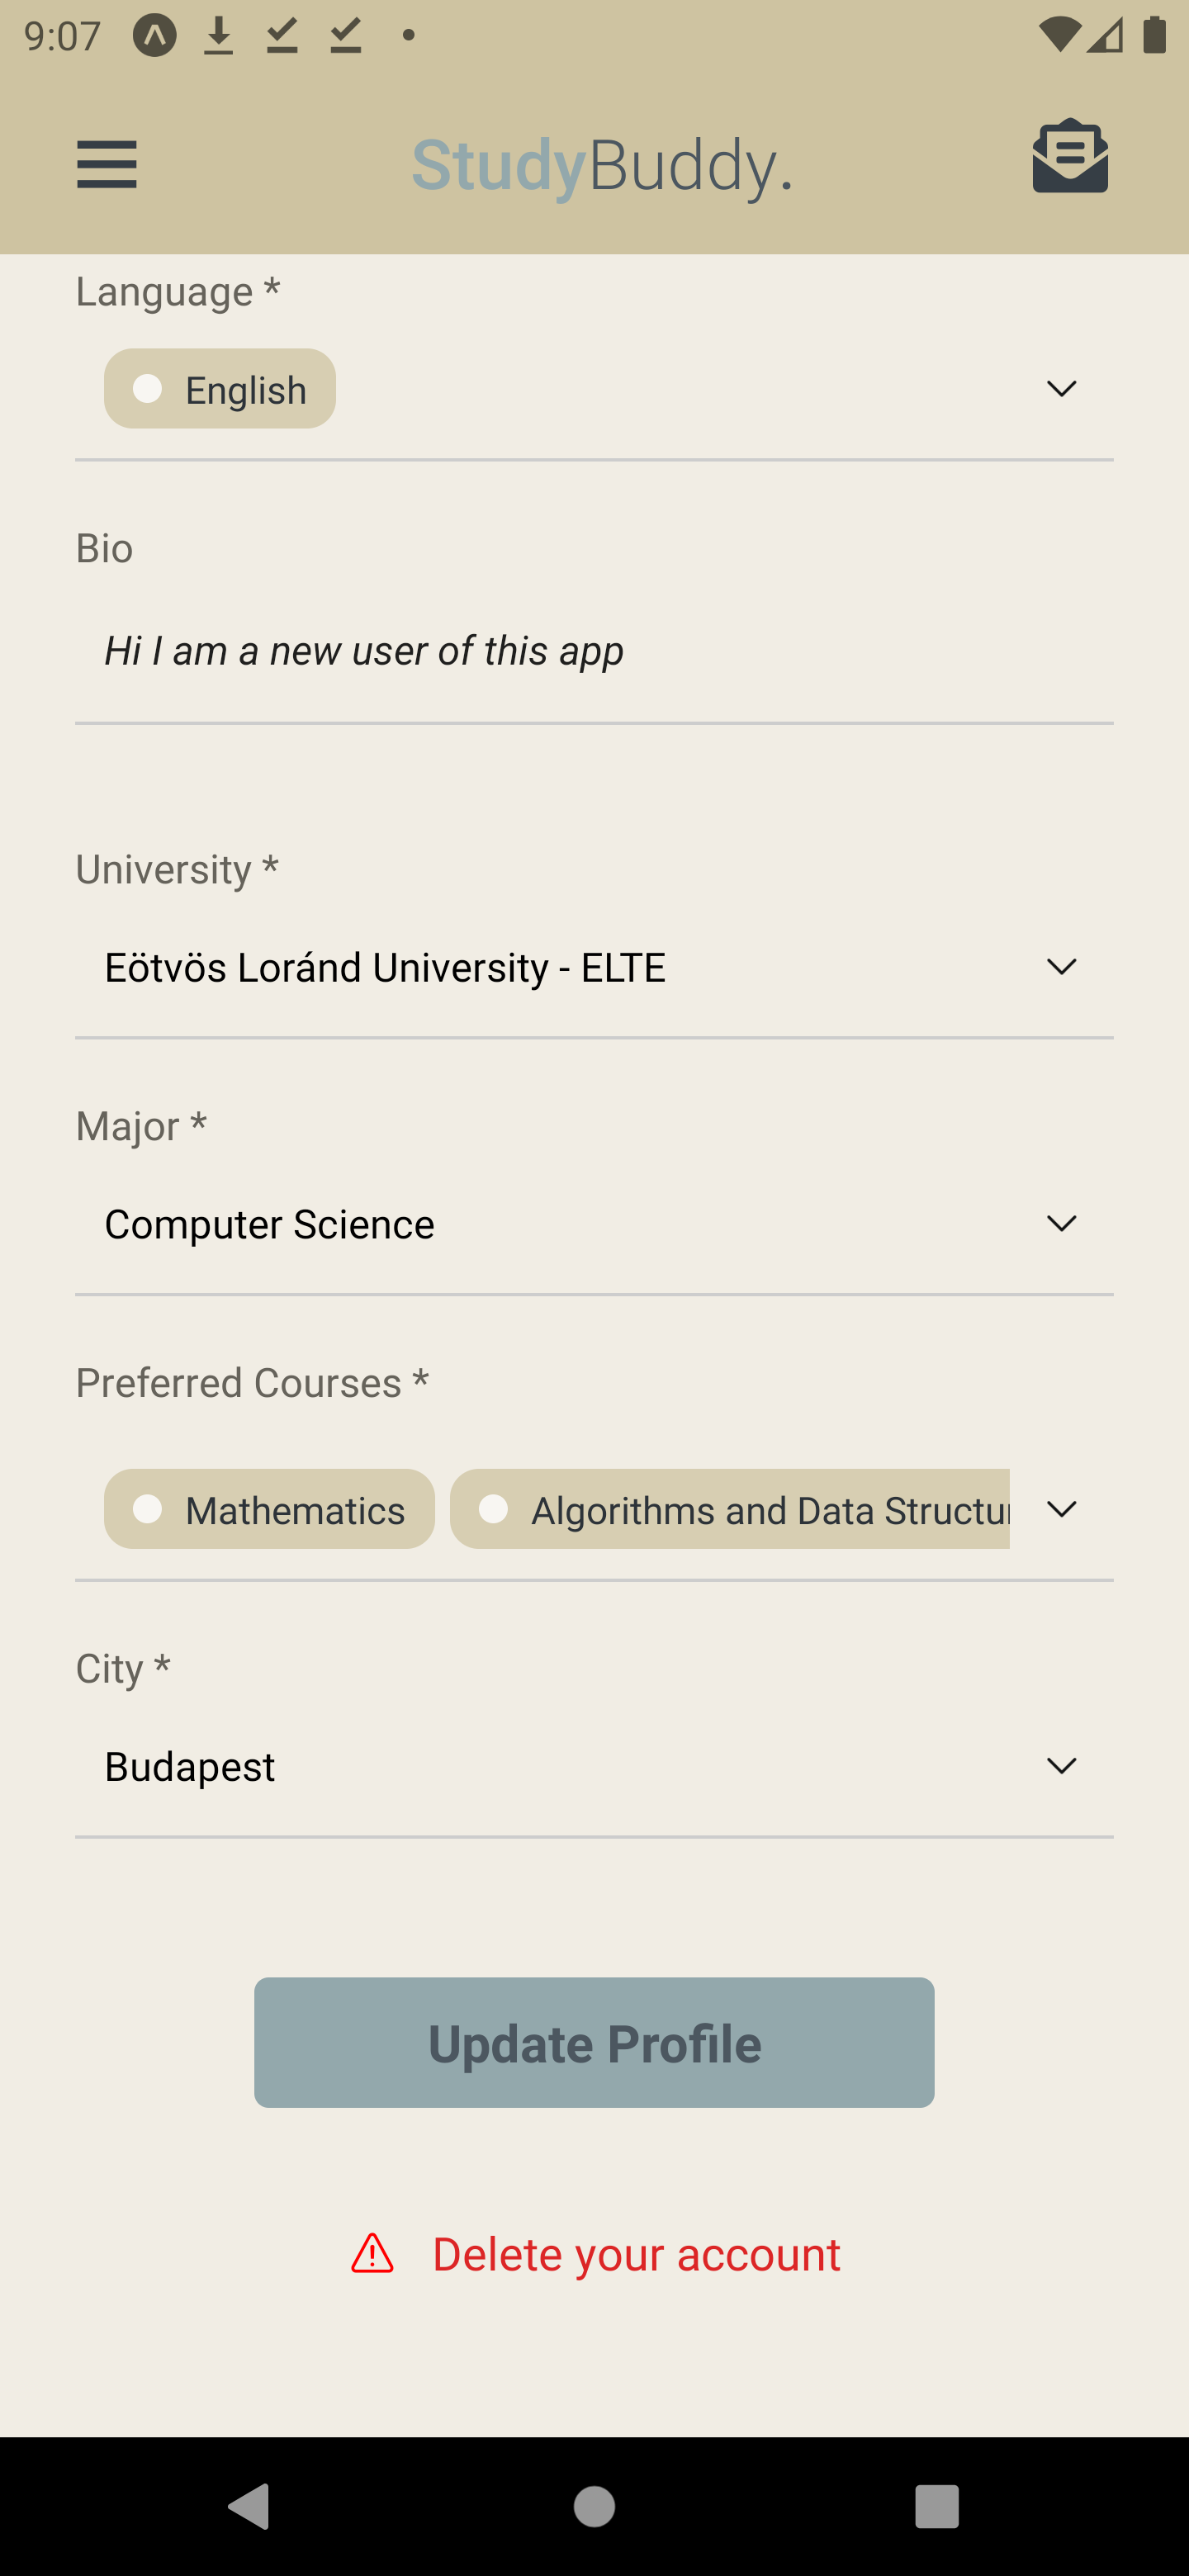
\includegraphics[width=0.45\linewidth, width=5cm, height=10cm]{images/snapshots/edit_profile_2.png}}
	\caption{Edit Profile}
	\label{fig:edit-profile-screen}
\end{figure}
\subsection{Matches Screen}
The Matches screen displays a list of buddies if available. If there are no buddies yet, a button is shown to navigate back to the home screen. In the list of buddies, users can click on a buddy to open a buddy info modal similar to \ref{fig:home-screen}, providing detailed information about the buddy. Each buddy listing includes message and delete buttons. Tapping the message button navigates the user to write a message, while the delete button removes the buddy from the list as shown in Figure~\ref{fig:matches-screen}
   \begin{figure}[H]
	\centering
		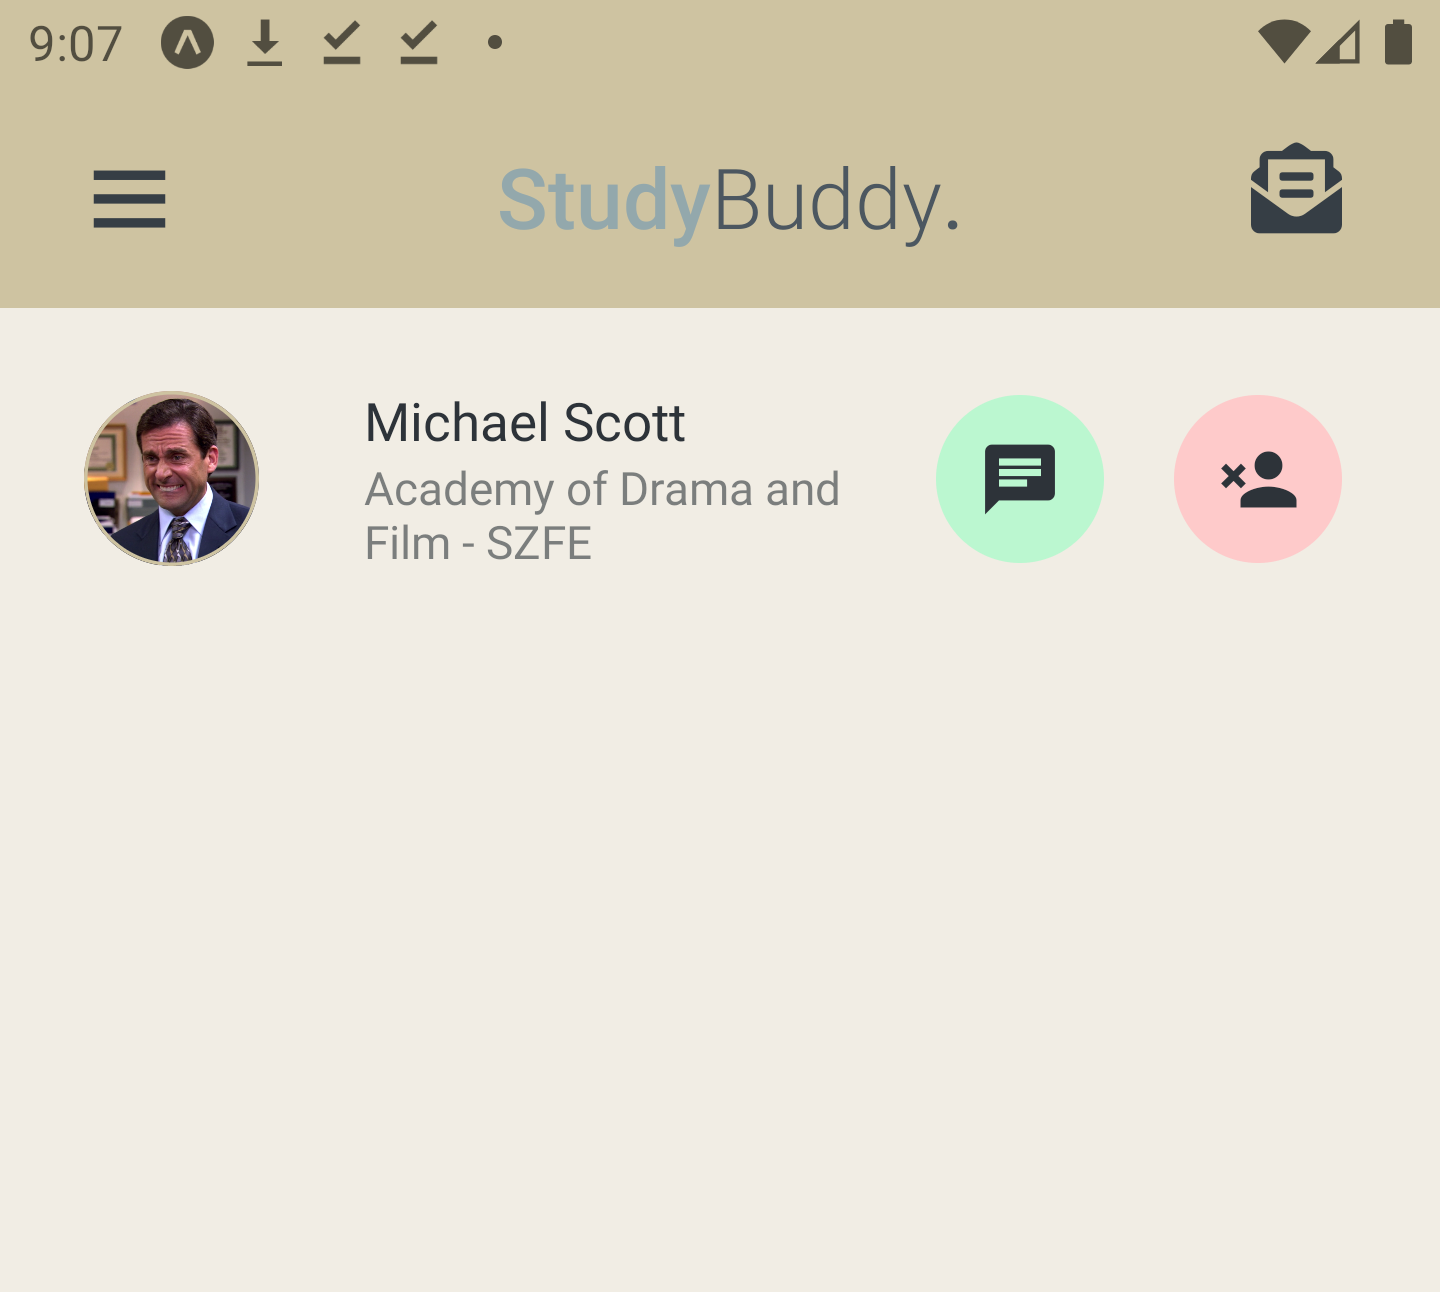
\includegraphics[width=0.45\linewidth, width=6cm, height=5cm]{images/snapshots/matches_screen.png}
        \caption{Matches Screen}
	\label{fig:matches-screen}
  \end{figure}
\subsection{Contact Us and Logout}
The Contact Us screen (figure~\ref{fig:contactus-screen}) provides developers' contact information for users who need assistance or wish to report problems. The Logout option, which is available in the drawer as shown in figure~\ref{fig:drawer}, triggers a prompt to confirm if the user wants to log out. Upon confirmation, users are navigated back to the login screen.
    \begin{figure}[H]
	\centering
		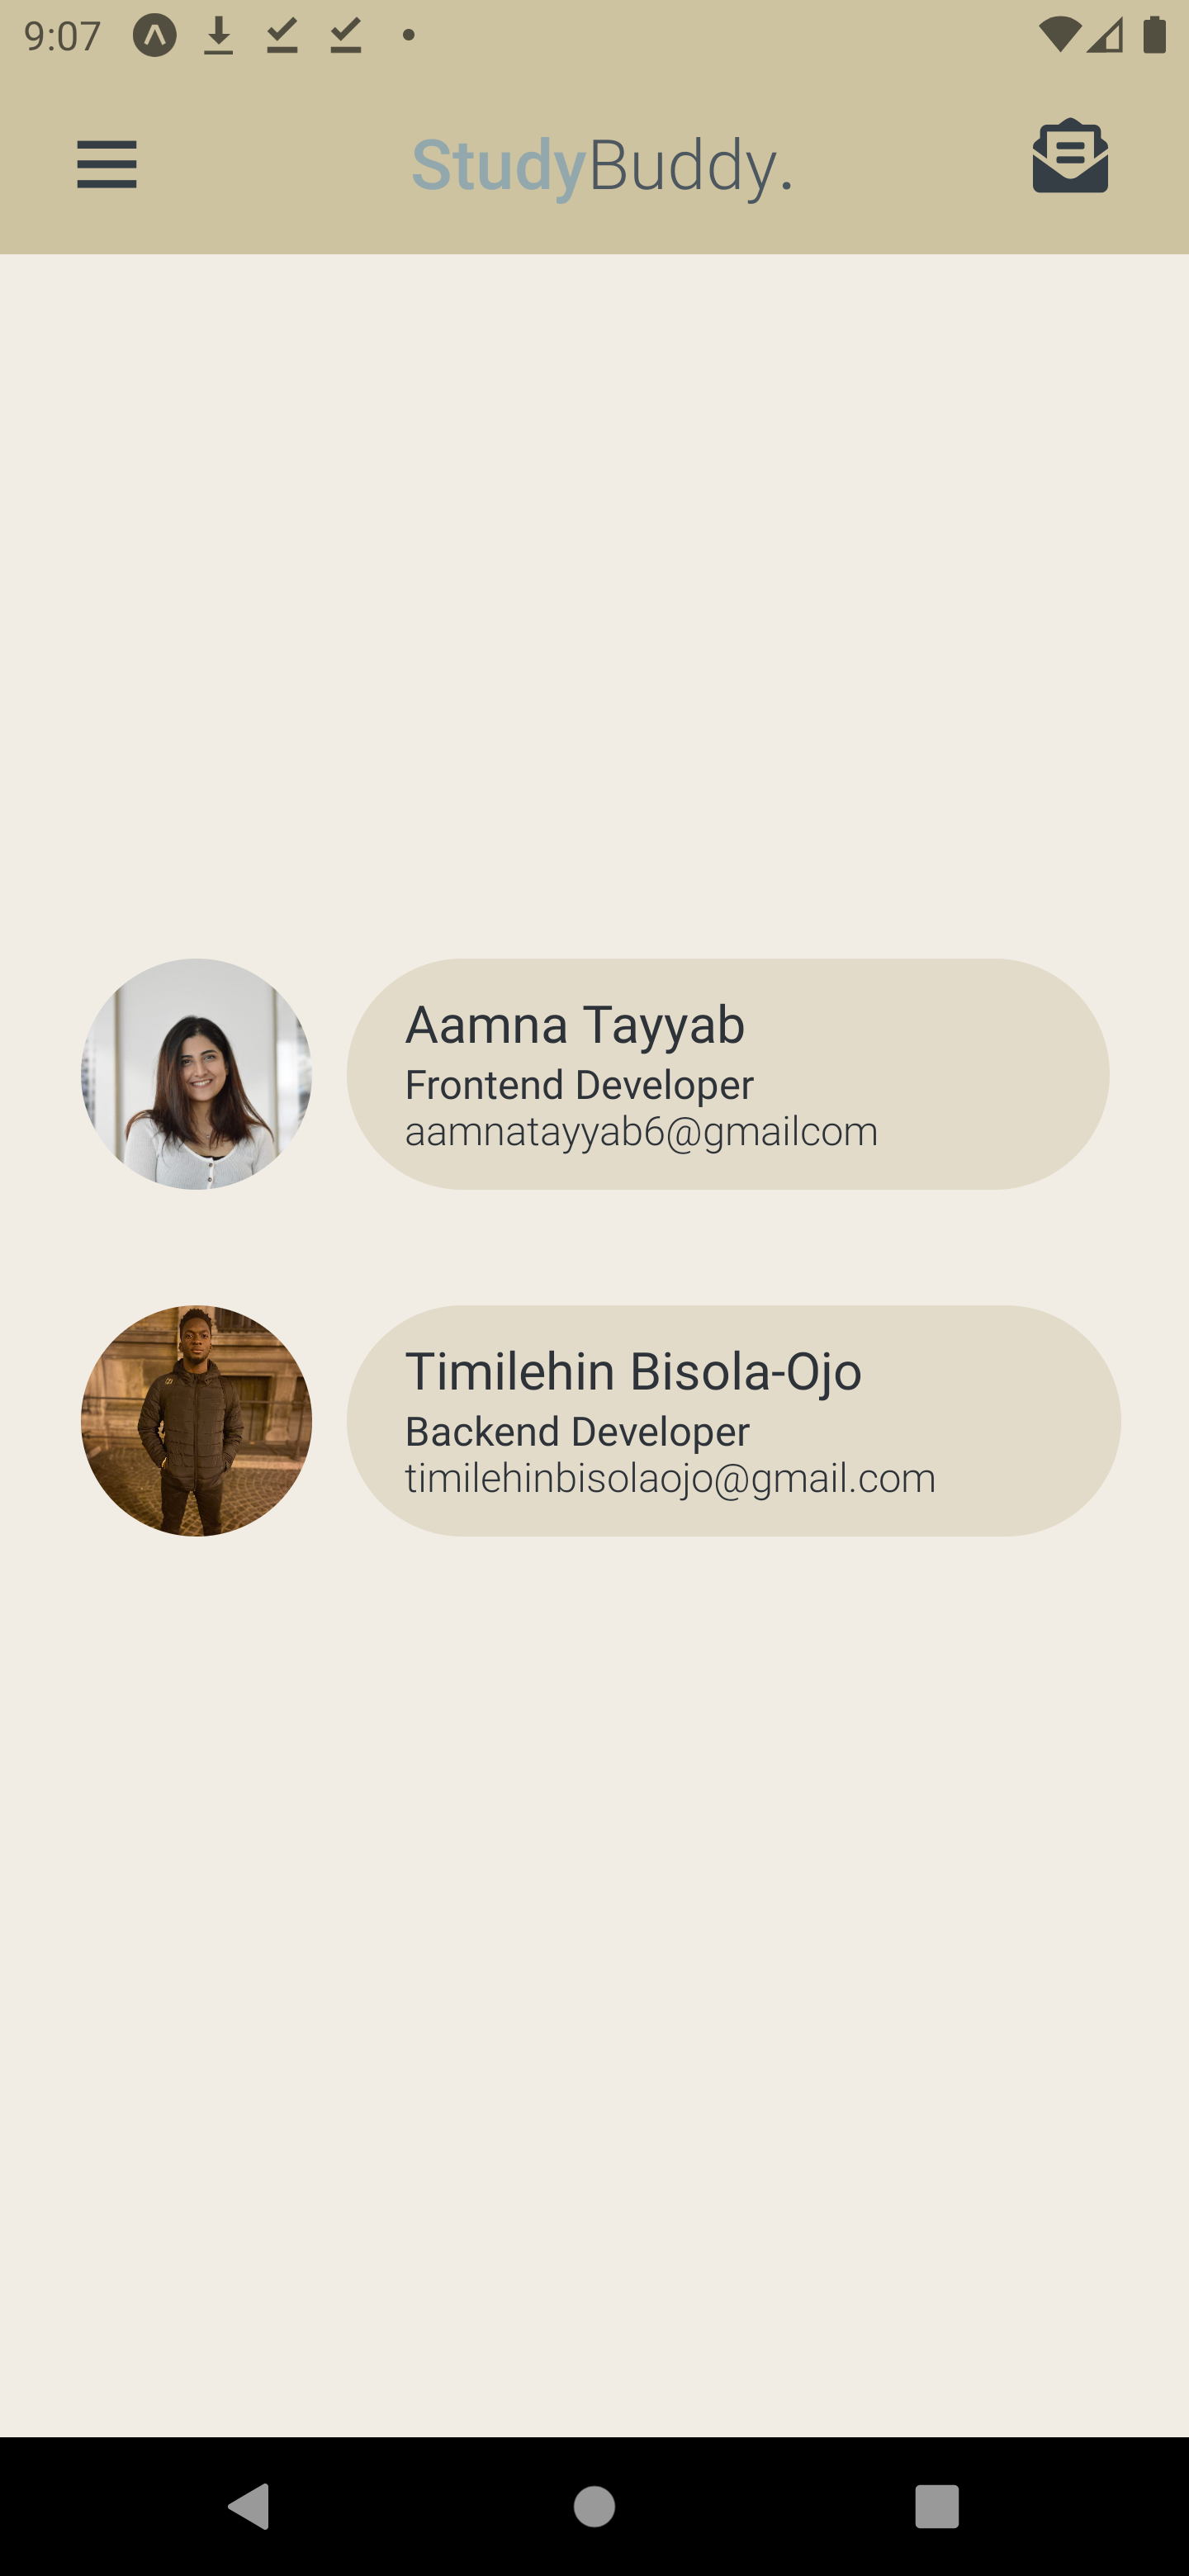
\includegraphics[width=0.45\linewidth, width=5cm, height=9cm]{images/snapshots/contact_us.png}
        \caption{Contact Us Screen}
	\label{fig:contactus-screen}
  \end{figure}
\bigskip
To manage daily app usage and server load, users are automatically logged out after 50 minutes of session. The swipe functionality ensures that unwanted interactions are minimized, making the implementation of a topic forum or group messaging less relevant. (Refer to Section \ref{sec:constraints})
\section{Terms and Conditions}\label{sec:tnc}
During Registration process, users are required to accept Terms and Conditions which are stated in this section. Users are responsible for maintaining the confidentiality of their login data, including email address and password. \\
By using this application, users agree to strictly comply with the terms and agreements and undertake to refrain from engaging in the following activities:
\begin{enumerate}
    \item Discrimination: Users must not discriminate based on age, ethnicity, color, religion, gender identity, sexual orientation, appearance, personal and political beliefs, or engage in any similar activities.
    \item Copyright Violations: Users must not engage in posting or sharing any content that violates copyright rules.
    \item Illegal Activities and Prohibited Content: Users must not engage in illegal activities or promote anything that violates community guidelines, such as selling or promoting drugs, pornography, or adult content.
    \item Personal Information: Users must not disseminate their personal and sensitive information to other users or third parties without proper consent.
    \item False or Misleading Statements: Users must not spread false, misleading, or deceptive statements or representations about the App, the Websites, or the Services.
    \item Not a Dating or Matrimonial Platform: Users should not treat this application as a dating or matrimonial platform.
\end{enumerate}
Each user is required to report any misconduct or abuse by other users to the creators of the app. In cases of hate speech, abusive behavior, or content dissemination, the creators reserves the right to permanently remove the user's account and take strict legal actions.

The terms and conditions, as well as the privacy policy, may be updated by the creators as the application evolves. Users are responsible for complying with the latest terms and conditions, and if they do not agree, they should cease using the application.
\subsection{Messaging System and Privacy Policy}
Our messaging system operates on an asynchronous model, where messages are fetched from the server only when the chat screen is mounted or when a new message is sent. This approach optimizes resource usage by minimizing unnecessary API calls and ensures that messages are retrieved and displayed efficiently, enhancing the overall user experience. The creators reserve the right to change the message exchanges to real-time chats in future updates.
\subsection{Privacy Policy Statement}
We collect necessary private information, such as name, email address, and location, to facilitate user interaction within our service. Optional sensitive information, like a profile picture and personal profile, can be provided to enhance profile visibility for potential study partners.
\subsection{Collection of User Data}
During registration, users will be asked to provide their personal email address. Additionally, users can select preferred courses and subjects to find suitable study partners. To improve the matching process, we may request additional information such as geolocation, university affiliation, and languages spoken fluently. However to uphold fairness and respect user privacy, we do not mandate the provision of age-related information during registration. Additionally, including a profile picture is optional, allowing users the choice to personalize their profiles at their discretion.
\subsection{How User Information is Used}
The application utilizes private and optional information to perform analysis and provide users with study buddy recommendation scores based on different preferences using OpenAI API (see section~\ref{sec:libraries}). All user-provided information is treated confidentially and used solely for managing accounts, finding suitable study partners, and providing customer support.

\subsection{Data Protection}
To safeguard user data from unauthorized access or disclosure, we employ security precautions. While we take measures to protect information, no system can guarantee 100 percent security. Users should also exercise caution when sharing personal information.
\subsection{Contact Us}
For any queries regarding our privacy policy or terms and conditions, please contact us via emails (aamnatayyab6@gmail.com or timilehinbisolaojo@gmail.com).
\section{Network}
The app operates on a network-dependent model, necessitating an active internet connection for full functionality. Users are required to have a stable Wi-Fi connection or cellular data connectivity to access and interact with the app's features. Similar to other messenger and social apps, StudyBuddy relies on network connectivity to send and receive data to and from the backend server.
\section{Quick Start Guide}\label{sec:qsg}
\subsection{Video Demonstration}
 In addition to the tutorial, a video demonstration showcasing the key functionalities of StudyBuddy is available. The videos provide a visual walk-through of the app's features, highlighting its user-friendly interface and collaborative capabilities. The videos for registration of user is available at this \href{https://youtu.be/qcr-2ob2LYc}{link}. The app usage video is available \href{https://youtu.be/TWF3gzYAzlM}{here}.
\section{Limitations and Constraints}\label{sec:constraints}
While using the Study Buddy app, it's important to be aware of certain limitations and constraints. These constraints are outlined below to provide users with a clear understanding of the app's functionalities and restrictions:
\begin{compactenum}
    \item \textbf{Platform Limitation:} The app was initially intended to be cross-platform; however, due to design considerations not aligning with iOS build guidelines, it is currently available only for Android devices. The Expo framework, although capable of building for iOS and web platforms, is optimized primarily for Android.
    \item \textbf{Swipe Functionality:} The app incorporates swipe functionality to minimize unwanted interactions and focus on individual matching between users. As a result, the implementation of features such as topic forums or group messaging was deemed less relevant and therefore not included in the app.
    \item \textbf{Geographic Restriction:} StudyBuddy is designed specifically for users in Hungary. Therefore, when selecting cities and universities within the app, only options from Hungary will be available in the respective drop-down menus. 
\end{compactenum}
\bigskip
By understanding these constraints, users can align their expectations with the app's current capabilities and intended usage. The StudyBuddy app aims to provide a streamlined and focused study partner finding experience, tailored to the Hungarian context.